\chapter{Modelos de Transporte}
\noindent

\section{Modelo de transporte lineal}

Sean $u,\omega,f : \left[0,T \right[ \times \R^N \to \R^N$ y $\omega_0: \left[0,T \right[ \times \R^N \to \R$. Los modelos que vamos a estudiar
se corresponden con la ecuación siguiente\footnote{Puede leerse $\di_x$ como divergencia respecto de $x$.}:
\begin{equation}\label{eq:ec10}
    \dfrac{\partial u}{\partial t} + \di_x(\overbrace{\omega:u}^{\text{flujo}}) + \omega_0 u = f
\end{equation}
Al final solo nos quedará un modelo de dos términos. El primer sumando es un vector porque $u$ es un campo vectorial. El tercer sumando también,
y $f$ es vectorial. Para que la ecuación tenga sentido, el sumando de en medio debe ser un vector\footnote{En otro caso estaría mal escrita la ecuación.}. 
Así, el argumento de dicho sumando debe ser una matriz\footnote{Repasar la Sección \ref{section:div}.}. Como la ecuación es vectorial, no hay una sola ecuación, hay $N$.
Componente a componente sería
$$\dfrac{\partial u_j}{\partial t} + (\di_x(\overbrace{\omega:u}^{\text{flujo}}))_j + \omega_0 u_j = f_j \quad 1 \leq j \leq N$$
Nos interesa ahora describir el sumando $\di_x(\omega:u)$. El argumento $\omega:u$ es el producto producto tensorial o producto exterior de vectores, habitualmente denotado por 
$\omega\otimes u$. Se corresponde con la siguiente matriz $(\omega_iu_j)_{1 \leq i,j \leq N}$. Ahora nos hacemos la siguiente pregunta: ¿qué sentido tiene, si lo tiene, la divergencia de una matriz\footnote{La de una función
escalar ya la conocemos.}? La idea será aplicar la definición columna a columna de la divergencia de un vector. \\

Partimos entonces de $(\di_x(\omega : u))_j$, para cierta columna $1 \leq j \leq N$, y entonces aplicamos el concepto de divergencia ya conocido:
$$(\di_x(\omega : u))_j = \sum_{i=1}^{N} \dfrac{\partial}{\partial x_i} (w_i u_j) = \sum_{i=1}^{N} \left[\dfrac{\partial w_i}{\partial x_i} u_j + w_i \dfrac{\partial u_j}{\partial x_i} \right] =$$
$$u_j\sum_{i=1}^{N} \dfrac{\partial w_i}{\partial x_i} + \sum_{i=1}^{N} w_i \dfrac{\partial u_j}{\partial x_i} = \di_x(\omega) u_j + (\omega \cdot \nabla_x) u_j$$
Ahora vienen las simplificaciones, porque el modelo genérico es muy complicado.

\subsection{Simplificaciones del modelo lineal}

Consideraremos 

$$
\boxed{
\begin{gathered}
f = 0 \\
\omega_0 = -\di_x(\omega)
\end{gathered}
}
$$

La primera simplificación significa que no vamos a considerar fuerza. Será el modelo homogéneo. Además, es importante
tener en cuenta que $\omega$ es conocida desde el principio. Es el campo (vectorial fijo) de velocidades asociado a nuestro sistema de partículas.
Sustituyendo estas simplificaciones en el modelo general, obtenemos
$$\dfrac{\partial u}{\partial t} + \di_x(\omega) u + (\omega \cdot \nabla_x) u + \omega_0 u = f \Longrightarrow 
\dfrac{\partial u}{\partial t} + (\omega \cdot \nabla_x) u = 0$$
Asociaremos a esta ecuación la siguiente condición inicial, para cierta $u_0 : \R^N \to \R^N$ conocida:
$$u(0,x) = u_0(x)$$
de tal manera que ya podemos definir el modelo de transporte lineal (simplificado):

\begin{definicion}[Modelo de Transporte Lineal Simplificado (MTLS)]
    \begin{equation}\label{eq:ec3}
        \begin{cases}
            \dfrac{\partial u}{\partial t} + (\omega \cdot \nabla_x) u = 0 \\
            u(0,x) = u_0(x)
        \end{cases}
    \end{equation}
\end{definicion}

\begin{observacion}
    En el caso en que $N>1$, se tiene:
    $$\omega = (\omega_1, \ldots, \omega_N), \quad \nabla_x = \left( \dfrac{\partial}{\partial x_1}, \ldots, \dfrac{\partial}{\partial x_N} \right)$$
    y el producto escalar queda:
    $$(\omega \cdot \nabla_x)u = \sum_{i=1}^{N} \omega_i \dfrac{\partial u}{\partial x_i}$$
    Si $N=1$, entonces:
    \begin{equation*}
        \begin{cases}
            \dfrac{\partial u}{\partial t} + \omega(t,x) \dfrac{\partial u}{\partial x} = 0 \\
            u(0,x) = u_0(x)
        \end{cases}
    \end{equation*}
    Y se usará la notación $u_t = \frac{\partial u}{\partial t}$ y $u_x = \frac{\partial u}{\partial x}$ indistintamente.
\end{observacion}

Para resolver el PVI \eqref{eq:ec3}, debemos resolver primeramente un problema auxiliar, conocido como \textit{sistema característico}, que consiste en
encontrar ciertas trayectorias que determinarán cómo será el transporte.

\newpage

\begin{definicion}[Sistema Característico]
    Viene determinado por la ecuación $$X'(t) = \omega(t,X(t))$$
    Las trayectorias soluciones de esta ecuación nos explican cómo son las curvas que siguen nuestras partículas en $\R^N$ si
    la velocidad a la que están sujetas dichas partículas es $\omega$. Para obtener una única solución, impondremos una condición inicial de la forma
    $X(s) = x \in \R^N$. Típicamente $s=0$. Así, consideramos el siguiente PVI:
    \begin{equation}\label{eq:ec2}
        \begin{cases}
            X'(t) = \omega(t,X(t)) \\
            X(s) = x \in \R^N \quad s \in \left[0, T \right[
        \end{cases}
    \end{equation}
\end{definicion}

Debemos resolver el problema \eqref{eq:ec2}~forzosamente para resolver \eqref{eq:ec3}. Nos situaremos entonces en las siguientes condiciones favorables:
\begin{itemize}
    \item[(H1)] $\omega$ es continua en los dos argumentos. Con esto nos garantizamos la existencia.
    \item[(H2)] $\omega$ es localmente Lipschitz en el segundo argumento (l.l. resp. de $x$). Juntando ambas cosas tenemos Cauchy-Peano y Picard-Lindelöf, es decir,
    existencia y unicidad local. Habitualmente esta segunda hipótesis se deducirá de ser la función $C_x^1$.
    \item[(H3)] El crecimiento de $\omega$ es sublineal. Con esto nos garantizaremos que la solución esté definida en $\left[0, T\right[$.
    $$\norma{\omega(t,x)} \leq A|x| + B; \quad A,B \in \R$$
    \item[(H4)] La aplicación \Func{\dfrac{\partial \omega_i}{\partial x_j}}{\left[0, T \right[ \times \R^N}{\R}{(t,x)}{\dfrac{\partial \omega_i}{\partial x_j}(t,x)} es continua para todo $i,j \in \{1, \ldots, N\}$.
\end{itemize} 

Con estas 4 hipótesis, \eqref{eq:ec2} tiene una única solución. Dicha solución se denotará en lo que sigue como $X(t;s,x)$, es decir,
siempre seguiremos la pista de la condición inicial, porque será esencial. Reescribiendo \eqref{eq:ec2} usando esta última notación nos queda:
\begin{equation}\label{eq:ec32}
    \left\{
    \begin{array}{l}
    X'(t)=\omega(t,X(t))\\[6pt]
    X(s)=x
    \end{array}
    \right.
    \quad
    \overset{X(t)\equiv X(t;s,x)}{\longleftrightarrow}
    \quad
    \left\{
    \begin{array}{l}
    \dfrac{\partial X}{\partial t}(t;s,x)
    =\omega(t,X(t;s,x))\\[6pt]
    X(s;s,x)=x
    \end{array}
    \right.
\end{equation}

\begin{teo}\label{teo:t3}
    Bajo las hipótesis (H1)$-$(H4), se satisface:
    \begin{itemize}
        \item[(i)] Fórmula de traslación característica:\label{ftc}
        $$X(t;\tau, X(\tau;s,x)) = X(t;s,x) \quad \forall t, \tau, s \in \left[0, T\right[, \quad \forall x \in \R^N$$

        \begin{figure}[H]
            \begin{center}
                \tikzset{every picture/.style={line width=0.75pt}} %set default line width to 0.75pt        

                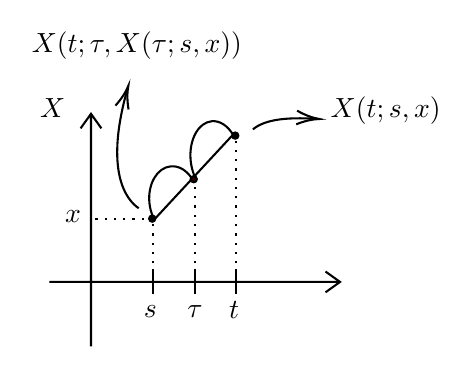
\begin{tikzpicture}[x=0.75pt,y=0.75pt,yscale=-1,xscale=1]
                %uncomment if require: \path (0,300); %set diagram left start at 0, and has height of 300

                %Shape: Axis 2D [id:dp3242275334401292] 
                \draw  (220,150) -- (360,150)(240,69) -- (240,181) (353,145) -- (360,150) -- (353,155) (235,76) -- (240,69) -- (245,76)  ;
                %Straight Lines [id:da6800909913200827] 
                \draw    (270,144) -- (270,156) ;
                %Straight Lines [id:da504363558290425] 
                \draw    (290,144) -- (290,156) ;
                %Straight Lines [id:da4011575225736249] 
                \draw    (310,144) -- (310,156) ;
                %Straight Lines [id:da4288458752818559] 
                \draw  [dash pattern={on 0.84pt off 2.51pt}]  (270,150) -- (270,119) ;
                %Straight Lines [id:da5200175588918502] 
                \draw  [dash pattern={on 0.84pt off 2.51pt}]  (269.98,119.83) -- (239.98,119.83) ;
                %Shape: Circle [id:dp34120311380094603] 
                \draw  [fill={rgb, 255:red, 0; green, 0; blue, 0 }  ,fill opacity=1 ] (268,119.5) .. controls (268,118.67) and (268.67,118) .. (269.5,118) .. controls (270.33,118) and (271,118.67) .. (271,119.5) .. controls (271,120.33) and (270.33,121) .. (269.5,121) .. controls (268.67,121) and (268,120.33) .. (268,119.5) -- cycle ;
                %Straight Lines [id:da41768238504122124] 
                \draw  [dash pattern={on 0.84pt off 2.51pt}]  (290,150) -- (290,99) ;
                %Straight Lines [id:da8451658517460895] 
                \draw    (269.5,121) -- (308,79.5) ;
                %Shape: Circle [id:dp23983039955771324] 
                \draw  [fill={rgb, 255:red, 47; green, 0; blue, 0 }  ,fill opacity=1 ] (288,100.5) .. controls (288,99.67) and (288.67,99) .. (289.5,99) .. controls (290.33,99) and (291,99.67) .. (291,100.5) .. controls (291,101.33) and (290.33,102) .. (289.5,102) .. controls (288.67,102) and (288,101.33) .. (288,100.5) -- cycle ;
                %Shape: Arc [id:dp02494682923156455] 
                \draw  [draw opacity=0] (269.98,118.83) .. controls (269.02,116.72) and (268.37,114.32) .. (268.13,111.74) .. controls (267.32,102.69) and (271.94,94.88) .. (278.46,94.3) .. controls (282.33,93.95) and (285.99,96.21) .. (288.5,100) -- (279.94,110.67) -- cycle ; \draw   (269.98,118.83) .. controls (269.02,116.72) and (268.37,114.32) .. (268.13,111.74) .. controls (267.32,102.69) and (271.94,94.88) .. (278.46,94.3) .. controls (282.33,93.95) and (285.99,96.21) .. (288.5,100) ;  
                %Curve Lines [id:da623468907736261] 
                \draw    (263,114.5) .. controls (257.09,110.56) and (246.33,96.92) .. (257.48,57.33) ;
                \draw [shift={(258,55.5)}, rotate = 106.31] [color={rgb, 255:red, 0; green, 0; blue, 0 }  ][line width=0.75]    (10.93,-3.29) .. controls (6.95,-1.4) and (3.31,-0.3) .. (0,0) .. controls (3.31,0.3) and (6.95,1.4) .. (10.93,3.29)   ;
                %Shape: Arc [id:dp26745949184759055] 
                \draw  [draw opacity=0] (289.71,98.58) .. controls (288.84,96.41) and (288.25,93.97) .. (288.01,91.37) .. controls (287.13,81.57) and (291.69,73.15) .. (298.21,72.56) .. controls (302.23,72.2) and (306.05,74.91) .. (308.6,79.34) -- (299.81,90.31) -- cycle ; \draw   (289.71,98.58) .. controls (288.84,96.41) and (288.25,93.97) .. (288.01,91.37) .. controls (287.13,81.57) and (291.69,73.15) .. (298.21,72.56) .. controls (302.23,72.2) and (306.05,74.91) .. (308.6,79.34) ;  
                %Straight Lines [id:da6666191987751137] 
                \draw  [dash pattern={on 0.84pt off 2.51pt}]  (310,150) -- (310,78) ;
                %Shape: Circle [id:dp19053748007169846] 
                \draw  [color={rgb, 255:red, 0; green, 0; blue, 0 }  ,draw opacity=1 ][fill={rgb, 255:red, 0; green, 0; blue, 0 }  ,fill opacity=1 ] (308,79.5) .. controls (308,78.67) and (308.67,78) .. (309.5,78) .. controls (310.33,78) and (311,78.67) .. (311,79.5) .. controls (311,80.33) and (310.33,81) .. (309.5,81) .. controls (308.67,81) and (308,80.33) .. (308,79.5) -- cycle ;
                %Curve Lines [id:da7070550816349991] 
                \draw    (318,76.5) .. controls (323.76,71.7) and (334.13,70.59) .. (348.22,71.39) ;
                \draw [shift={(350,71.5)}, rotate = 183.81] [color={rgb, 255:red, 0; green, 0; blue, 0 }  ][line width=0.75]    (10.93,-3.29) .. controls (6.95,-1.4) and (3.31,-0.3) .. (0,0) .. controls (3.31,0.3) and (6.95,1.4) .. (10.93,3.29)   ;

                % Text Node
                \draw (264,160) node [anchor=north west][inner sep=0.75pt]   [align=left] {$\displaystyle s$};
                % Text Node
                \draw (285,160) node [anchor=north west][inner sep=0.75pt]   [align=left] {$\displaystyle \tau $};
                % Text Node
                \draw (305,158) node [anchor=north west][inner sep=0.75pt]   [align=left] {$\displaystyle t$};
                % Text Node
                \draw (226,114) node [anchor=north west][inner sep=0.75pt]   [align=left] {$\displaystyle x$};
                % Text Node
                \draw (210,28) node [anchor=north west][inner sep=0.75pt]   [align=left] {$\displaystyle X( t;\tau ,X( \tau ;s,x))$};
                % Text Node
                \draw (354,59.5) node [anchor=north west][inner sep=0.75pt]   [align=left] {$\displaystyle X( t;s,x)$};
                % Text Node
                \draw (214,60) node [anchor=north west][inner sep=0.75pt]   [align=left] {$\displaystyle X$};


                \end{tikzpicture}
                \caption{Fórmula de traslación característica. Primero se llega hasta $\tau$, y luego hasta $t$. La fórmula nos dice que llegar de un tirón es como llegar haciendo paradas.}
                \label{fig:f21}
            \end{center}
        \end{figure}
        \item[(ii)] Fijados $s,t \in \left[0, T\right[$, la aplicación 
        \Func{T_s^t}{\R^N}{\R^N}{x}{T_s^t(x) = X(t;s,x)}
        es un difeomorfismo de clase $C^1(\R^N, \R^N)$ con operador inverso\footnote{También de clase $C^1(\R^N, \R^N)$.} 
        \Func{T_t^s}{\R^N}{\R^N}{x}{T_t^s(x) = X(s;t,x)}
        En palabras más sencillas, la inversa de ir de $s$ a $t$, es ir de $t$ a $s$ siguiendo la misma trayectoria\footnote{Podemos utilizar como ejemplo la situación de la Figura \ref{fig:f21}.}.
        \item[(iii)] El determinante jacobiano de las trayectorias características, es decir, 
        la aplicación dada por 
        \Func{J}{\left[0, T\right[^2 \times \R^N}{\R}{(t;s,x)}{J(t;s,x) = \begin{vmatrix}
            \dfrac{\partial X_i}{\partial x_j} (t;s,x) 
        \end{vmatrix}_{1 \leq i,j \leq N}}
        satisface\footnote{Podemos establecer un paralelismo entre esta expresión y la que se obtuvo de la variación del volumen del cubo en la motivación del concepto de divergencia (\ref{t1:interpretación}).} 
        $$\dfrac{\partial J}{\partial t}(t;s,x) = \di_x(\omega(t, X(t;s,x)))J(t;s,x)$$
        y además 
        $$J(t;t,x) = 1$$
        \item[(iv)] Si $\di_x(\omega) = 0$ (caso incompresible), el operador del apartado (ii), $T_s^t$, preserva la medida de Lebesgue.
    \end{itemize}
\end{teo}

\begin{proof}~
    \begin{itemize}
        \item[(i)] Por reducción al absurdo, si no fuera cierta la igualdad, habríamos encontrado dos soluciones distintas del mismo PVI \eqref{eq:ec32} 
        que coinciden en $X(\tau; s, x)$. Sustituyendo en la fórmula de traslación característica en $t = \tau$:
        $$X(\tau; \tau, X(\tau; s,x)) = X(\tau; s,x)$$
        Y tendríamos dos soluciones distintas del mismo PVI que coinciden en un punto, lo cual es una contradicción porque sabemos que este PVI
        tiene unicidad.
        \item[(ii)] Tenemos que probar que $T_s^t$ es una biyección, y luego que dicha biyección es bi-diferenciable (solo con la bicontinuidad tendríamos
        que es un homeomorfismo), y ver que ambos operadores son de clase $C^1$. \\

        Es trivial que son de clase $C^1$ con respecto al primer argumento por ser soluciones del PVI \eqref{eq:ec32}.
        Además, son de clase $C^1$ respecto a los otros dos argumentos por la hipótesis (H4), ya que dependía continua y diferenciablemente de los datos 
        iniciales. \\

        Para la inyectividad, basta con tener en cuenta que las imágenes de $T_s^t$ y $T_t^s$ son trayectorias características evolucionadas, y si 
        coinciden en algún punto, deben partir del mismo para evitar contradicción con la fórmula de traslación característica\footnote{Gráficamente lo vemos en la Figura \ref{fig:f22}.}. \\

        \begin{figure}
            \begin{center}
                \tikzset{every picture/.style={line width=0.75pt}} %set default line width to 0.75pt        

                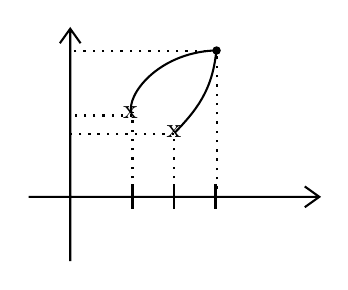
\begin{tikzpicture}[x=0.75pt,y=0.75pt,yscale=-1,xscale=1]
                %uncomment if require: \path (0,300); %set diagram left start at 0, and has height of 300

                %Shape: Axis 2D [id:dp3242275334401292] 
                \draw  (220,150) -- (360,150)(240,69) -- (240,181) (353,145) -- (360,150) -- (353,155) (235,76) -- (240,69) -- (245,76)  ;
                %Straight Lines [id:da6800909913200827] 
                \draw    (270,144) -- (270,156) ;
                %Straight Lines [id:da504363558290425] 
                \draw    (290,144) -- (290,156) ;
                %Straight Lines [id:da4011575225736249] 
                \draw    (310,144) -- (310,156) ;
                %Straight Lines [id:da4288458752818559] 
                \draw  [dash pattern={on 0.84pt off 2.51pt}]  (270,150) -- (270,109) ;
                %Straight Lines [id:da5200175588918502] 
                \draw  [dash pattern={on 0.84pt off 2.51pt}]  (269.98,110.83) -- (239.98,110.83) ;
                %Straight Lines [id:da12444846828280065] 
                \draw  [dash pattern={on 0.84pt off 2.51pt}]  (290,150) -- (290,121) ;
                %Straight Lines [id:da2984178356461328] 
                \draw  [dash pattern={on 0.84pt off 2.51pt}]  (289.98,119.83) -- (239.98,119.83) ;
                %Shape: Circle [id:dp3001811327779722] 
                \draw  [fill={rgb, 255:red, 0; green, 0; blue, 0 }  ,fill opacity=1 ] (309,79.5) .. controls (309,78.67) and (309.67,78) .. (310.5,78) .. controls (311.33,78) and (312,78.67) .. (312,79.5) .. controls (312,80.33) and (311.33,81) .. (310.5,81) .. controls (309.67,81) and (309,80.33) .. (309,79.5) -- cycle ;
                %Straight Lines [id:da6340522878310485] 
                \draw  [dash pattern={on 0.84pt off 2.51pt}]  (310.5,150.5) -- (310.5,78.5) ;
                %Straight Lines [id:da7786265993123673] 
                \draw  [dash pattern={on 0.84pt off 2.51pt}]  (309.98,79.83) -- (239.98,79.83) ;
                %Curve Lines [id:da9873085816340168] 
                \draw    (269.5,109.5) .. controls (267,101) and (282,81) .. (309,79.5) ;
                %Curve Lines [id:da7083634369024402] 
                \draw    (290.5,119) .. controls (300,109) and (309,99) .. (310.5,78) ;

                % Text Node
                \draw (264,105) node [anchor=north west][inner sep=0.75pt]   [align=left] {x};
                % Text Node
                \draw (285,114) node [anchor=north west][inner sep=0.75pt]   [align=left] {x};


                \end{tikzpicture}
                \caption{Inyectividad. Si las dos características llegan al mismo punto, necesariamente deben partir del mismo punto. Las cruces denotan que esas características no son compatibles.}
                \label{fig:f22}
            \end{center}
        \end{figure}

        Respecto a la sobreyectividad, nos preguntamos si $\exists x \in \R^N$ tal que $y = X(t;s,x)$. Es fácil ver\footnote{Gráficamente lo vemos en la Figura \ref{fig:f23}.} que 
        dicho $x$ será $x = X(s;t, y)$.  \\

        \begin{figure}
            \begin{center}
                \tikzset{every picture/.style={line width=0.75pt}} %set default line width to 0.75pt        

                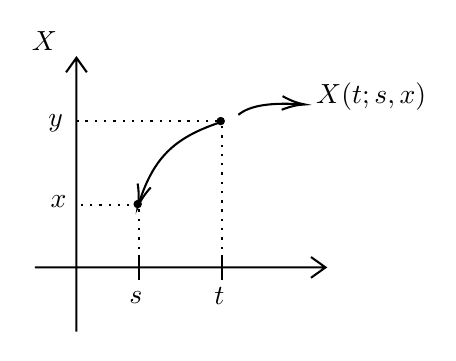
\begin{tikzpicture}[x=0.75pt,y=0.75pt,yscale=-1,xscale=1]
                %uncomment if require: \path (0,300); %set diagram left start at 0, and has height of 300

                %Shape: Axis 2D [id:dp3242275334401292] 
                \draw  (220,150) -- (360,150)(240,49) -- (240,181) (353,145) -- (360,150) -- (353,155) (235,56) -- (240,49) -- (245,56)  ;
                %Straight Lines [id:da6800909913200827] 
                \draw    (270,144) -- (270,156) ;
                %Straight Lines [id:da4011575225736249] 
                \draw    (310,144) -- (310,156) ;
                %Straight Lines [id:da4288458752818559] 
                \draw  [dash pattern={on 0.84pt off 2.51pt}]  (270,150) -- (270,119) ;
                %Straight Lines [id:da5200175588918502] 
                \draw  [dash pattern={on 0.84pt off 2.51pt}]  (269.98,119.83) -- (239.98,119.83) ;
                %Shape: Circle [id:dp34120311380094603] 
                \draw  [fill={rgb, 255:red, 0; green, 0; blue, 0 }  ,fill opacity=1 ] (268,119.5) .. controls (268,118.67) and (268.67,118) .. (269.5,118) .. controls (270.33,118) and (271,118.67) .. (271,119.5) .. controls (271,120.33) and (270.33,121) .. (269.5,121) .. controls (268.67,121) and (268,120.33) .. (268,119.5) -- cycle ;
                %Straight Lines [id:da6666191987751137] 
                \draw  [dash pattern={on 0.84pt off 2.51pt}]  (310,150) -- (310,78) ;
                %Shape: Circle [id:dp19053748007169846] 
                \draw  [color={rgb, 255:red, 0; green, 0; blue, 0 }  ,draw opacity=1 ][fill={rgb, 255:red, 0; green, 0; blue, 0 }  ,fill opacity=1 ] (308,79.5) .. controls (308,78.67) and (308.67,78) .. (309.5,78) .. controls (310.33,78) and (311,78.67) .. (311,79.5) .. controls (311,80.33) and (310.33,81) .. (309.5,81) .. controls (308.67,81) and (308,80.33) .. (308,79.5) -- cycle ;
                %Curve Lines [id:da7070550816349991] 
                \draw    (318,76.5) .. controls (323.76,71.7) and (334.13,70.59) .. (348.22,71.39) ;
                \draw [shift={(350,71.5)}, rotate = 183.81] [color={rgb, 255:red, 0; green, 0; blue, 0 }  ][line width=0.75]    (10.93,-3.29) .. controls (6.95,-1.4) and (3.31,-0.3) .. (0,0) .. controls (3.31,0.3) and (6.95,1.4) .. (10.93,3.29)   ;
                %Curve Lines [id:da691035537947874] 
                \draw    (311,79.5) .. controls (288.58,86.81) and (277.56,95.55) .. (270.07,119.15) ;
                \draw [shift={(269.5,121)}, rotate = 286.7] [color={rgb, 255:red, 0; green, 0; blue, 0 }  ][line width=0.75]    (10.93,-3.29) .. controls (6.95,-1.4) and (3.31,-0.3) .. (0,0) .. controls (3.31,0.3) and (6.95,1.4) .. (10.93,3.29)   ;
                %Straight Lines [id:da31623284526739026] 
                \draw  [dash pattern={on 0.84pt off 2.51pt}]  (308,79.5) -- (240,79.5) ;

                % Text Node
                \draw (264,160) node [anchor=north west][inner sep=0.75pt]   [align=left] {$\displaystyle s$};
                % Text Node
                \draw (305,158) node [anchor=north west][inner sep=0.75pt]   [align=left] {$\displaystyle t$};
                % Text Node
                \draw (226,114) node [anchor=north west][inner sep=0.75pt]   [align=left] {$\displaystyle x$};
                % Text Node
                \draw (354,59.5) node [anchor=north west][inner sep=0.75pt]   [align=left] {$\displaystyle X( t;s,x)$};
                % Text Node
                \draw (217,35) node [anchor=north west][inner sep=0.75pt]   [align=left] {$\displaystyle X$};
                % Text Node
                \draw (225,75) node [anchor=north west][inner sep=0.75pt]   [align=left] {$\displaystyle y$};


                \end{tikzpicture}
                \caption{Sobreyectividad. Recorremos hacia delante partiendo de $x$ en el instante $s$ y llegamos a $y$ en el instante $t$, luego $y=X(t;s,x)=T_s^t(x)$. Para volver, hacemos el recorrido hacia atrás: partimos de $y$ en el instante $t$ y retrocedemos hasta $x$ en el instante $s$,
                o sea $x=X(s;t,y)=T_t^s(y)$}
                \label{fig:f23}
            \end{center}
        \end{figure}

        Así, falta comprobar que son inversas la una de la otra, lo cual se deduce de que 
        $$T_t^s(T_s^t(x)) = T_t^s(X(t;s,x)) = X(s;t,X(t;s,x)) \stackrel{(i)}{=} X(s;s,x) = x$$
        $$T_s^t(T_t^s(x)) = T_s^t(X(s;t,x)) = X(t;s,X(s;t,x)) \stackrel{(i)}{=} X(t;t,x) = x$$

        \item[(iii)] Se deja como ejercicio.
        \item[(iv)] Por hipótesis, sustituyendo en (iii)
        $$\dfrac{\partial J}{\partial t}(t;s,x) = \di_x(\omega)J(t;s,x) = 0 \stackrel{J(t;t,x)}{\Longrightarrow} J \equiv 1$$
        Para ver que $T_s^t$ preserva la medida de Lebesgue, tomamos una función $f$ integrable y vemos que 
        $$\int_{\R^N} f(x) dx \stackrel{x = T_s^t(y)}{=} \int_{\R^N} f(T_s^t(y)) \overbrace{J}^{1} dy = \int_{\R^N} f(T_s^t(y)) dy$$
    \end{itemize}
\end{proof}

A partir de ahora, recordamos dos teorías para tratar el modelo de transporte simplificado (mtls). Recordemos que dicho modelo se corresponde con el PVI \eqref{eq:ec3}. Las dos 
variantes que tenemos son:
\begin{enumerate}
    \item Teoría fuerte / clásica, considerando $u_0 \in C^1(\R^N)$.
    \item Teoría débil, considerando $u_0 \in L_{loc}^1(\R^N)$.
\end{enumerate}

\subsection{Teoría clásica para el MTLS}

\begin{teo}[Existencia y Unicidad de Soluciones Clásicas de \eqref{eq:ec3}]\label{teo:t1}
    Bajo las hipótesis (H1)-(H4) sobre $\omega$ y dado un dato inicial $u_0 \in C^1(\R^N)$, el PVI \eqref{eq:ec3} \underline{admite una única solución}
    $u \in C^1(\left[0, T \right[ \times \R^N)$ que viene dada por 
    $$\boxed{u(t,x) = u_0(X(0;t,x))}$$
\end{teo}

Teniendo esto en cuenta, escribimos el sistema característico, resolvemos el sistema, obtendremos las trayectorias características, las recorremos a la inversa\footnote{Es decir, la evaluamos en $0$.}, y una vez tengamos ese valor, metemos esa expresión en el dato inicial.
Realmente entonces lo único que hay que hacer es encontrar las trayectorias características, es decir, resolver \eqref{eq:ec2}. \\

\begin{ejercicio}
    Resuélvanse los siguientes problemas de transporte lineal:
    \begin{enumerate}
        \item[(i)] $N=1$. $\begin{cases}
            \dfrac{\partial u}{\partial t} + x \dfrac{\partial u}{\partial x} = 0 \\
            u(0,x) = x
        \end{cases} \quad (x \in \R)$

        Tenemos que comprobar que se satisfacen las hipótesis (H1)-(H4) (sencillo en este caso), y luego resolver el sistema característico asociado al 
        campo de velocidades, es decir, \eqref{eq:ec2}. En este caso, $\omega(t,x) = x$, luego debemos resolver\footnote{Usaremos para resolver los sistemas característicos la notación $X(t) \equiv X(t;s,x)$ cuando la condición inicial de \eqref{eq:ec2} sea $X(s) = x$.}
        $$\begin{cases}
            \dfrac{\partial X}{\partial t}(t;s,x)
            =\omega(t,X(t;s,x)) = X(t;s,x)\\[6pt]
            X(s;s,x)=x
        \end{cases}$$
        y nos queda un problema unidimensional con una ecuación diferencial de variables separadas cuya solución es conocida: $X(t;s,x) = xe^{t-s}$. Como $u_0(x) = x \in C^1(\R)$, 
        por el Teorema \ref{teo:t1}, la única solución del PVI es, teniendo en cuenta que $X(0;t,x) = xe^{-t}$, la siguiente:
        $$u(t,x) = u_0(X(0;t,x)) = u_0(xe^{-t}) = xe^{-t} \in C^1(\left[0, T \right[ \times \R)$$
        \item[(ii)] $N=2$.
        $\begin{cases}
            \dfrac{\partial u}{\partial t} \overbrace{- 2y \dfrac{\partial u}{\partial x} + 2x \dfrac{\partial u}{\partial y}}^{(\omega \cdot \nabla_x) u} = 0 \\
            u(0,x,y) = x + y
        \end{cases}$

        En este caso, $u : \left[0, T \right[ \times \R^2 \to \R$ y $\omega : \left[0, T \right[ \times \R^2 \to \R^2$.

        % TODO: Terminar
    \end{enumerate}
\end{ejercicio}

Probamos ahora el Teorema \ref{teo:t1}.

\begin{proof}
    Primero demostraremos la existencia, y luego la unicidad.
    \begin{itemize}
        \item[$(i)$] Existencia. \\
        
        El dato inicial se satisface trivialmente. Ahora, veamos que se cumple \eqref{eq:ec3}. Basta con derivar y aplicar la regla de la cadena:
        $$\dfrac{\partial}{\partial t}(u_0(X(0;t,x))) = \nabla_x u_0(X(0;t,x)) \cdot \dfrac{\partial}{\partial t}(X(0;t,x))$$
        Además
        $$\left[(\omega \cdot \nabla_x)(u_0(X(0;t,x))) \right]_j = \sum_{i=1}^{N} \omega_i \dfrac{\partial}{\partial x_i} \left( u_0^j (X(0;t,x)) \right) = $$
        $$\sum_{i=1}^{N} \omega_i \sum_{k=1}^{N} \dfrac{\partial u_0^j}{\partial x_k} \left((X(0;t,x)) \right) \dfrac{\partial X_k}{\partial x_i}(0;t,x) =$$
        $$\nabla_x u_0(X(0;t,x)) \cdot ((\omega \cdot \nabla_x) X(0;t,x)) \quad 1 \leq j \leq N$$

        Falta entonces sumar ambos y ver que dicha suma es $0$. Así pues
        $$\left( \dfrac{\partial}{\partial t} + (\omega \cdot \nabla_x) \right)(u_0(X(0;t,x))) = \nabla_x u_0(X(0;t,x)) \cdot \left( \dfrac{\partial}{\partial t} + (\omega \cdot \nabla_x) \right) X(0;t,x)$$
        Para ver que esto es $0$, recurrimos a la fórmula de traslación característica (\ref{ftc}). Derivamos con respecto a $\tau$:
        $$0 = \dfrac{\partial X}{\partial \tau} (t;\tau;X(\tau;s,x)) + \overbrace{\nabla_x X}^{J \text{ (jacobiana)}} (t;\tau,X(\tau;s,x)) \cdot \dfrac{\partial X}{\partial t} (\tau; s,x)$$
        y viendo que\footnote{Por el sistema característico.} 
        $$\dfrac{\partial X}{\partial t}(\tau; s,x) = \omega(\tau; X(\tau;s,x))$$
        y evaluando en $\tau = s$:
        $$0 = \dfrac{\partial X}{\partial s} (t;s;\overbrace{X(s;s,x)}^{x}) + \overbrace{\nabla_x X}^{J \text{ (jacobiana)}} (t;s,\overbrace{X(s;s,x)}^{x}) \cdot \overbrace{\dfrac{\partial X}{\partial t} (s; s,x)}^{\omega(s,x)}$$
        Por lo tanto, evaluamos en $t=0$, inferimos que 
        $$\nabla_x u_0(X(0;t,x)) \cdot \overbrace{\left( \dfrac{\partial}{\partial t} + (\omega \cdot \nabla_x) \right) X(0;t,x)}^{0} = 0$$
        por lo que en efecto $u(t,x) = u_0(X(0;t,x))$ es solución. 

        \item[$(ii)$] Unicidad. \\
        
        Sea $u$ una solución cualquiera de \eqref{eq:ec3}. Nuevamente aplicando la regla de la cadena:
        $$\dfrac{d}{dt}(u(t,X(t;0,x))) = \dfrac{\partial u}{\partial t}(t,X(t;0,x)) + \nabla_x u (t,X(t;0,x)) \cdot \dfrac{\partial X}{\partial t}(t;0,x) = $$
        $$\dfrac{\partial u}{\partial t} (t,X(t;0,x)) + \nabla_x u(t,X(t;0,x)) \cdot \omega(t,X(t;0,x)) \stackrel{(*)}{=} 0$$
        donde en $(*)$ se ha usado que $u$ es solución de \eqref{eq:ec3}. \\

        De la última igualdad se deduce que la solución se transporta a lo largo de las trayectorias características\footnote{De ahí su nombre: se llama modelo de transporte porque el campo de velocidades $\omega$ mueve las partículas a lo largo de las trayectorias características, 
        transportando los valores iniciales de $u$ sin modificarlos.}. 
        En particular
        $$u(t;X(t;0,x)) = \overbrace{u(0,X(0;0,x))}^{u_0(x)} \quad \forall t$$
        
        Dado un dato inicial, lo que hace el operador de transporte es llevarlo por las trayectorias características. \\

        Para concluir la unicidad, hacemos el siguiente cambio de variable:
        $$u_0(X(0;t,y)) = u(t,y)\Longleftarrow y = \overbrace{X(t;0,x)}^{T_0^t(x)} \Longrightarrow x = T_t^{0}(y) = X(0;t,y)$$
        O sea, cualquier solución de \eqref{eq:ec3} tiene la forma anterior, por lo que se tiene la unicidad. \qedhere
    \end{itemize}
\end{proof}

En resumen, tomamos el dato inicial, y lo evaluamos en las trayectorias características hacia atrás. Así se soluciona el problema de transporte.

% Teoría débil mañana. Mucho más débil. Ni siquiera son continuas las soluciones, solo L^1_loc.

% Miércoles mínimo 2 horas, lo más complicado del Bloque a nivel teórico. Estudiaremos X' = \omega(t,X) porque hará falta para el bloque de fluidos
% sin las hipótesis (H1)-(H4)
% En el segundo argumento será logarítmica Lipschitz, más débil que localmente Lipschitz, y en el primero no va a ser ni continua.

\subsection{Teoría débil para el MTLS}

Consideraremos funciones $\varphi = \varphi(t,x)$ con $\varphi \in C^1_c(\left[0,T \right[ \times \R^N)$\footnote{Recordamos estos conceptos. Sea $\Omega\in\mathcal{P}(\R^N)$ y $f:\Omega\to\R$. Se define el soporte de $f$ como el cierre, relativo a $\Omega$, del conjunto de puntos en los que $f$ no se anula, es decir:
$$\sop f = \overline{\{x \in \Omega : f(x) \neq 0\}} \subset \Omega$$ Se dice que $f$ tiene soporte compacto en $\Omega$ si $\sop f$ es un subconjunto compacto de $\Omega$. En particular definimos 
$$C_c^1(\Omega) = \{f : \Omega \to \R : f \in C^1(\Omega) \quad \land \quad \sop f \text{ es compacto}\}$$ En nuestro caso consideramos una componente (temporal) más ($N+1$ en total), y $\Omega = \left[0,T\right[ \times \R^N \subset \R^{N+1}$. 
Como las funciones test $\varphi$ tienen soporte compacto en $\Omega=\left[0,T \right[\times\R^N$, existe $t_0 < T$ tal que $\varphi$ se anula en $\left]t_0, T \right[$. Por tanto, extendiéndola hacia la derecha de manera continua como $\varphi(t,x) = 0$, tenemos que $\varphi(T,x)=0$ para todo $x\in\R^N$.}. \\ 

La formulación débil será:

$$\int_0^T \int_{\R^N} \left[ \dfrac{\partial u}{\partial t} + (\omega \cdot \nabla_x) u \right] \varphi\,dx\,dt = 0$$

Entonces, hacemos lo siguiente. Por un lado
$$\int_0^T \int_{\R^N} \left[ \dfrac{\partial u}{\partial t} \right] \varphi\,dx\,dt \stackrel{Fubini | Partes}{=} 
\int_{\R^N} (u \cancelto{0}{\varphi(T,x)} - \overbrace{u \varphi(0,x))}^{u(0,x)\varphi(0,x)} \,dx - \int_{\R^N} \int_{0}^{T} u \dfrac{\partial \varphi}{\partial t} \,dt\,dx = $$
$$\boxed{- \int_{\R^N} \int_{0}^{T} u \dfrac{\partial \varphi}{\partial t} \,dt\,dx - \int_{\R^N}u_0(x) \varphi(0,x)\,dx}$$

y por el otro
$$\sum_i \int_{0}^{T} \int_{R^N} \omega_i \dfrac{\partial u_j}{\partial x_i} \varphi \,dx\,dt \stackrel{F|P}{=} 
\sum_i \int_{0}^{T} \left[ \cancelto{0}{\omega_i \varphi u_j |_{|x| \nearrow \infty}} - \int_{\R^N} u_j \dfrac{\partial}{\partial x_i} (\omega_i \varphi) \,dx\right] = $$
$$- \sum_i \int_{0}^{T} \int_{\R^N} u_j \left[ \dfrac{\partial \omega_i}{\partial x_i} \varphi + \omega_i \dfrac{\partial \varphi}{\partial x_i} \right] \,dx\,dt = $$
$$\boxed{- \int_{0}^{T} \int_{\R^N} \overbrace{\left[ \di_x(\omega) \varphi + (\omega \cdot \nabla_x) \varphi \right]}^{\di_x(\omega \varphi)} u \,dx\,dt}$$

Juntando ambas cosas, la formulación débil asociada a \eqref{eq:ec3} es \eqref{eq:ec4}:

\begin{definicion}[Formulación débil del MTLS]
    \begin{equation}\label{eq:ec4}
        - \int_{0}^{T} \int_{\R^N} \left[ \dfrac{\partial \varphi}{\partial t} + \di_x(\omega \varphi) \right] u \,dx\,dt = \int_{\R^N} u_0(x) \varphi(0,x)\,dx
    \end{equation}
\end{definicion}

Para facilitar las cosas, supondremos el caso de un fluido incompresible, es decir, $\di_x(\omega) = 0$. De esta manera\footnote{Consultar el primer punto del apartado ii) del Ejercicio \ref{ejercicio:ej12}. Aquí se ha aplicado con $f = \varphi(t, \cdot)$ y $F = \omega(t, \cdot)$
fijando el tiempo $t$, y teniendo en cuenta que la propiedad es válida para cualquier dimensión $N \geq 1$, no solo para $N = 3$.}:
$$\di_x(\omega \varphi) = \cancelto{0}{\di_x(\omega) \varphi} + (\omega \cdot \nabla_x) \varphi = (\omega \cdot \nabla_x) \varphi$$
y llegamos a la formulación con que trabajaremos:
\begin{definicion}[Formulación débil simplificada del MTLS]
    \begin{equation}\label{eq:ec5}
        - \int_{0}^{T} \int_{\R^N} \left[ \dfrac{\partial \varphi}{\partial t} + (\omega \cdot \nabla_x) \varphi \right] u \,dx\,dt = \int_{\R^N} u_0(x) \varphi(0,x)\,dx
    \end{equation}
\end{definicion}

Podemos definir entonces qué es una solución débil de \eqref{eq:ec3}:

\begin{definicion}[Solución débil de \eqref{eq:ec3}]\label{definicion:d1}
    Sean $\omega_i \in L_{loc}^{\infty}(\left[0,T \right[ \times \R^N)$, con $1 \leq i \leq N$, y $u_0 \in L_{loc}^{1}(\R^N)$.
    Diremos que $u \in L^1_{loc}(\left[0,T \right[ \times \R^N)$ es una \underline{solución débil} de \eqref{eq:ec3} si satisface \eqref{eq:ec5} para todo 
    $\varphi \in C_c^1(\left[0,T \right[ \times \R^N)$.
\end{definicion}

Veamos entonces un teorema (que asume hipótesis muy convenientes, del mismo modo que el Teorema \ref{teo:t1}) para encontrar estas soluciones débiles:

\begin{teo}[Existencia y Unicidad de Soluciones Débiles de \eqref{eq:ec3}]
    Sea $\omega : \left[0,T \right[ \times \R^N \to \R^N$ una función que satisface (H1)-(H4) y tal que $\di_x(\omega) = 0$. Sea también $u_0 \in L_{loc}^{1}(\R^N)$.
    Entonces \eqref{eq:ec3}~\underline{admite una única solución}\footnote{Por la Definición \ref{definicion:d1}, esta será de la forma $u \in L^1_{loc}(\left[0,T \right[ \times \R^N)$.} que 
    viene dada por 
    $$\boxed{u(t,x) = u_0(X(0;t,x))}$$ 
\end{teo}

\begin{observacion}
    Vemos que tanto con la formulación fuerte como con la débil, la solución de \eqref{eq:ec3}~tiene la misma forma.
\end{observacion}

\begin{proof}
    \begin{itemize}
        \item[$(i)$] Existencia. \\
        
        Nos preguntamos si 
        $$\hspace{-1cm} \overbrace{-\int_{0}^{T} \int_{\R^N} \left[ \dfrac{\partial \varphi}{\partial t} + (\omega \cdot \nabla_x) \varphi \right](t,x) u_0(X(0;t,x))\,dx\,dt}^{I}
        \stackrel{?}{=} \int_{\R^N} \varphi(0,x) u_0(x)\,dx \quad \forall \varphi \in C_c^1(\left[0,T \right[ \times \R^N)$$
        Para responder a la pregunta hacemos el siguiente cambio de variable: $y = X(0;t,x)$\footnote{Al aplicar el teorema de cambio de variable con $y=X(0;t,x)$, tenemos que 
        $dx=|J(t;0,y)|\,dy$. Por el Teorema \ref{teo:t3}, apartado (iii), como $\di_x(\omega)=0$, se deduce que $\frac{\partial J}{\partial t}(t;0,y)=0$. Además, por dicho apartado se tiene que $J(0;0,y)=1$. Por tanto, como $J$ es constante respecto de la primera
        variable $t$, $J(t;0,y) = J(0;0,y) =1$ y, en consecuencia, $dx=dy$.}, de tal manera que nos queda
        $$I = -\int_{0}^{T} \int_{\R^N} \left[ \dfrac{\partial \varphi}{\partial t} + (\omega \cdot \nabla_x) \varphi \right] (t,X(t;0,y)) u_0(y)\,dy\,dt$$
        Definimos $\psi(t,y) = \varphi(t,X(t;0,y))$, y nos queda
        $$I = -\int_{0}^{T} \int_{\R^N} \dfrac{d \psi}{dt} u_0(y) \,dy\,dt = -\int_{\R^N} (\cancelto{0}{\psi(T,y)} - \psi(0,y)) u_0(y) \,dy\,dt =$$
        $$\int_{\R^N} \psi(0,y) u_0(y) \,dy\,dt$$
        Respondemos afirmativamente a la pregunta que nos hemos hecho, por lo que queda probada la existencia.

        \item[$(ii)$] Unicidad. Por reducción al absurdo, supongamos que $u_1$ y $u_2$ son soluciones débiles. Definimos la diferencia $v = u_1 - u_2$. Entonces
        $$-\int_{0}^{T} \int_{\R^N} \left[ \dfrac{\partial \varphi}{\partial t} + (\omega \cdot \nabla_x) \varphi \right](t,x) v(t,x) \,dx\,dt = 0 \quad \forall \varphi \in C_c^1(\left[0, T \right[ \times \R^N)$$
        Podríamos pensar en aplicar el lema fundamental del cálculo de variaciones, pero $v$ no es continua, solo $L^1_{loc}$, aunque el lema fundamental también
        sirve en este caso. Para ubicarnos en esta situación, consideramos el siguiente problema:
        $$\begin{cases}
            \dfrac{\partial \varphi}{\partial t} + (\omega \cdot \nabla_x) \varphi = \psi \\
            \varphi(T,x) = 0
        \end{cases}$$
        donde $\psi$ es una función test arbitraria. El Ejercicio \ref{ejercicio:ej25} demuestra la unicidad.
        Si encontrásemos dos soluciones distintas, diferirían en un conjunto de medida nula, por lo que concluye la demostración. \qedhere
    \end{itemize}
\end{proof}

\begin{ejercicio}\label{ejercicio:ej25} % TODO: Hacer
    Sea $\varphi(t,x) = \int_{T}^{t} \psi(s, X(s;t,x)) \,ds$.
    La forma de encontrar la solución si tiene segundo miembro no negativo es integrar el segundo miembro a través de las trayectorias características.
\end{ejercicio}

\newpage

\begin{observacion}~
    \begin{itemize}
        \item Se puede integrar desde $t$ hasta $T$ y poner el signo $-$.
        \item Es obvio que se verifica la condición inicial.
    \end{itemize}
\end{observacion}

Terminada la teoría débil, tenemos el siguiente ejercicio también:

\begin{ejercicio} % TODO: Hacer
    Consideramos un fluido compresible, es decir, $\di_x(\omega) \neq 0$. Entonces se cumple que 
    $$-\int_{0}^{T} \int_{\R^N} \left[ \dfrac{\partial \varphi}{\partial t} + \di_x(\omega \varphi) \right](t,x) u(t,x) \,dx\,dt = \int_{\R^N} \varphi(0,x) u_0(x) \,dx \quad \forall \varphi \in C_c^1(\left[0, T \right[ \times \R^N)$$
\end{ejercicio}

\begin{observacion}
    La principal diferencia es que ahora, al aplicar el teorema de cambio de variable, el determinante del jacobiano $|J|$ ya no es uno. Ahora la relación
    entre la divergencia y el jacobiano es la siguiente:
    $$\dfrac{\partial J}{\partial t} = \di_x(\omega) J$$
\end{observacion}

El teorema anterior se puede demostrar para el caso de fluidos compresibles, siguiendo los mismos pasos, y considerando
$$\varphi(t,x) = \int_{T}^{t} \psi(s,X(s;t,x)) e^{\displaystyle\int_{t}^{s} \di_x(\omega (\tau; X(\tau; t,x))) \,d \tau}\,ds$$

\subsection{Preparación para el bloque de fluidos}

Hasta ahora habíamos usado que $\omega$ era continua, lo cual facilitaba bastante las cosas. Ahora $\omega$ será menos ``generoso''. \\

Consideramos el siguiente problema de trayectorias características:
\begin{equation}\label{eq:ec6}
    \begin{cases}
        X'(t) = \omega(t,X(t)) \\
        X(0) = x \in \R^N
    \end{cases}
\end{equation}

Necesitaremos una serie de conceptos, que definimos a continuación:
\begin{definicion}[Campo Vectorial Logarítmicamente Lipschitziano]
    Diremos que un campo vectorial $f : \R^N \to \R^N$ es logarítmicamente lipschitziano (abreviado en adelante por LL) en $\R^N$, denotado por $LL(\R^N)$ si 
    $\exists C > 0$ tal que 
    $$|f(x) - f(y)| \leq C |x-y|(1-\log^{*}|x-y|)$$
    donde 
    $$\log^{*}(z) = \begin{cases}
        \log(z) &\quad 0 < z \leq 1 \\
        0 &\quad z > 1
    \end{cases}$$
    Gráficamente esta última función $\log^{*}(z)$ es la siguiente:

    \begin{figure}
        \begin{center}
            \tikzset{every picture/.style={line width=0.75pt}} %set default line width to 0.75pt        

            \begin{tikzpicture}[x=0.75pt,y=0.75pt,yscale=-1,xscale=1]
            %uncomment if require: \path (0,300); %set diagram left start at 0, and has height of 300

            %Shape: Axis 2D [id:dp7966055758022831] 
            \draw  (221,150) -- (420.67,150)(239.67,60) -- (239.67,251) (413.67,145) -- (420.67,150) -- (413.67,155) (234.67,67) -- (239.67,60) -- (244.67,67)  ;
            %Straight Lines [id:da015899118604729257] 
            \draw    (289.67,139) -- (289.67,161) ;
            %Straight Lines [id:da7754339207403739] 
            \draw [color={rgb, 255:red, 243; green, 0; blue, 0 }  ,draw opacity=1 ]   (289.67,150) -- (397.67,150) ;
            \draw [shift={(399.67,150)}, rotate = 180] [color={rgb, 255:red, 243; green, 0; blue, 0 }  ,draw opacity=1 ][line width=0.75]    (10.93,-3.29) .. controls (6.95,-1.4) and (3.31,-0.3) .. (0,0) .. controls (3.31,0.3) and (6.95,1.4) .. (10.93,3.29)   ;
            %Curve Lines [id:da7496613728346398] 
            \draw [color={rgb, 255:red, 0; green, 62; blue, 255 }  ,draw opacity=1 ]   (289.67,150) .. controls (241.39,150.63) and (245.98,201.73) .. (243.22,244.51) .. controls (243.1,246.25) and (242.98,247.97) .. (242.84,249.68) ;
            \draw [shift={(242.67,251.67)}, rotate = 275.19] [color={rgb, 255:red, 0; green, 62; blue, 255 }  ,draw opacity=1 ][line width=0.75]    (10.93,-3.29) .. controls (6.95,-1.4) and (3.31,-0.3) .. (0,0) .. controls (3.31,0.3) and (6.95,1.4) .. (10.93,3.29)   ;

            % Text Node
            \draw (295,156) node [anchor=north west][inner sep=0.75pt]   [align=left] {$\displaystyle 1$};
            \end{tikzpicture}
        \end{center}
    \end{figure}

\end{definicion}

\begin{observacion}
    Para distancias pequeñas estamos corrigiendo la condición de lipschitzianidad. Para distancias grandes ($>1$), tenemos la condición de lipschitzianidad
    tal y como la conocemos hasta ahora. \\

    Ser lipschitziano es más fuerte que ser logarítmicamente lipschitziano. Es decir, se puede ser logarítmicamente lipschitziano sin ser lipschitziano.
    De esta manera Picard-Lindelöf ya no nos sirve. \\

    Definiendo \Func{\lm}{\left] 0, 1 \right]}{\R}{r}{\lm(r) = r(1-\log(r))}
    y \Func{\lm^{*}}{\R^{+}}{\R}{r}{\lm^{*}(r) = r(1-\log^{*}(r))} 
    para ver que se tiene también la continuidad, si $r \to 0 \Longrightarrow \lm(r) \to 0$. Se puede ver por L'Hôpital por ejemplo. \\
    
    Así, la condición LL implica la continuidad. \\

    Usaremos que $\lm^{*}$ es creciente en $\Rmas$ (basta derivar y ver que es creciente en dicho intervalo).
\end{observacion}

\begin{ejercicio}\label{ejercicio:ej22} % TODO: HACER
    Verificar que el crecimiento de $\lm^{*}$ es sublineal. Concretamente:
    $$\lm^{*}(r) \leq - \log(\varepsilon) r + \varepsilon, \quad 0 < \varepsilon < \dfrac{1}{e}$$
\end{ejercicio}

Vamos a ver que la única trayectoria característica que resuelve \eqref{eq:ec6} lo hace con formulación integral. Es decir, 
si tenemos una solución de \eqref{eq:ec6}, también lo será de la siguiente ecuación integral:

\begin{equation}
    X(t) = x + \int_{0}^{t} \omega(s,X(s))\,ds
\end{equation}

Bastaría cambiar $L^1_{loc}$ por continuidad para tener existencia y unicidad de \eqref{eq:ec6}, donde la solución sería $C^1$. Más adelante 
veremos que cuando lleguemos al bloque de fluidos y a la ecuación de Euler, la condición será $L^1_{loc}$. \\

Resumimos lo anterior en el siguiente teorema:

\begin{teo}
    Sea $\omega : \left[ 0, T \right[ \times \R^N \to \R^N$ un campo vectorial localmente integrable en la primera variable, y LL en la segunda variable.
    Entonces \underline{existe una única solución continua}, $X \in C(\left[0, T \right[)$ del PVI \eqref{eq:ec6}. 
\end{teo}


\begin{proof}
    La demostración es una especie de reconstrucción del teorema de Picard. Construiremos las iterantes de Picard, veremos que están bien definidas
    y generan una sucesión que pasa bien al límite, y el límite es el que buscamos. \\

    \begin{itemize}
        \item[(i)] Existencia. \\
        
        Definimos recursivamente
        \begin{equation}\label{eq:ec7}
            \begin{cases}
                X_{n+1}(t) = x + \displaystyle\int_{0}^{t} \omega(s,X_n(s))\,ds \quad n \geq 0 \\
                X_0 \equiv x
            \end{cases}
        \end{equation}
        Ahora veamos que está bien definido \eqref{eq:ec7}. El caso $n=0$ está trivialmente bien definido. Para $n=1$:
        $$X_1 = x + \displaystyle\int_{0}^{t} \omega(s,X_0(s))\,ds = x + \displaystyle\int_{0}^{t} \omega(s,x)\,ds$$
        Sea ahora $I=\left[0,T\right[$. Por hipótesis, para cada $x\in\mathbb{R}^N$
        fijo, se tiene que
        \[
        \omega(\cdot,x)\in L^1_{\mathrm{loc}}(I,\mathbb{R}^N).
        \]
        Fijado $0<T_0<T$ arbitrario, como $[0,T_0]$ es un
        compacto contenido en $I$, resulta que
        \[
        \int_0^{T_0}|\omega(s,x)|\,ds<\infty.
        \]

        Por tanto, para todo $t\in[0,T_0]$, aplicando la
        desigualdad triangular:
        \[
        |X_1(t)|\leq |x|+\int_0^t|\omega(s,x)|\,ds
        \leq |x|+\int_0^{T_0}|\omega(s,x)|\,ds<\infty.
        \]

        Además, $X_1$ es continua, pues la integral indefinida
        de una función localmente integrable es absolutamente
        continua en cada intervalo compacto\footnote{Visto en Análisis Matemático II.}. Como $T_0<T$ es
        arbitrario, y la composición de una función constante con una función absolutamente continua es absolutamente continua (luego continua), concluimos que $X_1\in C(I,\mathbb{R}^N)$. \\

        Ahora argumentamos inductivamente. Supuesto que $X_n(t)$ está bien definida y es continua, probamos esta misma propiedad para $X_{n+1}(t)$.
        Como
        $$\left|\int_{0}^{t} \omega(s,X_n(s))\,ds \right| \leq \int_{0}^{T_0} |\omega(s,X_n(s))|\,ds$$
        y ahora el ``truco'' está en restar y sumar dentro del argumento del valor absoluto la cantidad $\omega(s,x)$, es decir:
        $$\int_{0}^{T_0} |\omega(s,X_n(s))|\,ds \leq \int_{0}^{T_0} |\omega(s,X_n(s)) - \omega(s,x)|\,ds + \int_{0}^{T_0} |\omega(s,x)|\,ds
        \stackrel{LL}{\leq}$$
        $$C\int_{0}^{T_0} \lm^{*}(|X_n(s) - x|)\,ds + \overbrace{\int_{0}^{T_0} |\omega(s,x)|\,ds}^{<\infty \text{ pq } \omega \in L^1_{loc}}$$
        Ahora como $\lm^{*}(|X_n(s) - x|)$ es continua (composición de continuas) en un compacto ($[0,T_0]$), por el Teorema de Weierstrass 
        tiene máximo, pongamos $M = \max_{0 \leq s \leq T_0} |X_n(s) - x|$. Análogamente, como la segunda integral es finita, pongamos
        que su valor es $M_{T_0}$, y nos queda que 
        $$C\int_{0}^{T_0} \lm^{*}(|X_n(s) - x|)\,ds + \int_{0}^{T_0} |\omega(s,x)|\,ds \leq C \int_{0}^{T_0} \lm^{*}(M)\,ds + M_{T_0} \leq$$
        $$C \lm^{*}(M)T_0 + M_{T_0} < \infty$$
        Ahora usaremos el criterio de la mayorante de Weierstrass (para series convergentes). La idea consiste en estudiar:
        $$|X_{n+1}(t) - X_n(t)| = \left| \int_{0}^{t} \left[ \omega(s,X_n(s)) - \omega(s,X_{n-1}) \right] \,ds \right| \leq$$
        $$\int_{0}^{t} |\omega(s,X_n(s)) - \omega(s,X_{n-1}(s))|\,ds \stackrel{LL}{\leq} C \int_{0}^{t} \lm^{*}(|X_n(s) - X_{n-1}(s)|)\,ds$$
        Por el Ejercicio \ref{ejercicio:ej22}, se tiene que 
        $$\lm^{*}(|X_n(s) - X_{n-1}(s)|) \leq a_{\varepsilon} |X_n(s) - X_{n-1}(s)| + \varepsilon, \quad a_{\varepsilon} = -\log(\varepsilon)$$
        y juntándolo con la última acotación superior:
        $$C \int_{0}^{t} \lm^{*}(|X_n(s) - X_{n-1}(s)|)\,ds \leq C \varepsilon t + C a_{\varepsilon} \int_{0}^{t} |X_n(s) - X_{n-1}(s)|\,ds$$
        A su vez con el último integrando podemos hacer una acotación análoga:
        $$|X_n(s) - X_{n-1}(s)| \leq C \varepsilon s + C a_{\varepsilon} \int_{0}^{s} |X_{n-1}(\tau) - X_{n-2}(\tau)|\,d \tau$$
        y repetiendo este proceso hasta llegar a la primera diferencia ($X_1 - X_0$), obtenemos
        $$C \varepsilon s + C a_{\varepsilon} \int_{0}^{s} |X_{n-1}(\tau) - X_{n-2}(\tau)|\,d \tau \leq $$
        $$C \varepsilon t + C a_{\varepsilon} \left[ \dfrac{C \varepsilon t^2}{2} + Ca_{\varepsilon} \int_{0}^{t} \int_{0}^{s} 
        \overbrace{|X_{n-1}(\tau) - X_{n-2}(\tau)|}^{C \varepsilon \tau + C a_\varepsilon \int_{0}^{\tau} |X_{n-2}(\sigma) - X_{n-3}(\sigma)|\,d \sigma}\,d \tau \, ds  \right] =$$
        $$C \varepsilon t + C^2 \varepsilon a_\varepsilon \dfrac{t^2}{2} + C^2 a^2_\varepsilon
        \left[ C \varepsilon \dfrac{t^3}{6} + C a_\varepsilon \int_{0}^{t} \int_{0}^{s} \int_{0}^{\tau} |X_{n-2}(\sigma) - X_{n-3}(\sigma)| d \sigma \right] = $$
        $$C \varepsilon t + C^2 \varepsilon a_\varepsilon \dfrac{t^2}{2} + C^3 \varepsilon a^2_\varepsilon \dfrac{t^3}{6} + C^3 a_\varepsilon^3 \int_{0}^{t} \int_{0}^{s} \int_{0}^{\tau}
        |X_{n-2}(\sigma) - X_{n-3}(\sigma)|\,d \sigma$$
        y en general esta expresión se escribe como sigue:
        $$\varepsilon \sum_{k=0}^{n-1} \dfrac{c^{k+1} t^{k+1} a_\varepsilon^k}{(k+1)!} + C^n a^n_\varepsilon \int_{0}^{t} \overbrace{\cdots}^{n)} \int_{0}^{s} |X_1(s) - \overbrace{X_0(s)}^{x}|\,ds$$
        y esta primera integral a su vez se escribe como
        $$|X_1(s) - x| = \int_{0}^{s} \omega(\tau, x)\,d \tau \leq \int_{0}^{T_0} \omega(\tau, x)\, d \tau \leq M_{T_0}$$
        Así pues, recapitulando, tenemos que 
        $$C \varepsilon s + C a_{\varepsilon} \int_{0}^{s} |X_{n-1}(\tau) - X_{n-2}(\tau)|\,d \tau \leq $$
        $$\varepsilon \sum_{k=0}^{n-1} \dfrac{c^{k+1} t^{k+1} a_\varepsilon^k}{(k+1)!} + C^n a^n_\varepsilon \int_{0}^{t} \overbrace{\cdots}^{n)} \int_{0}^{s} |X_1(s) - \overbrace{X_0(s)}^{x}|\,ds <$$
        $$\varepsilon C t \sum_{k=0}^{n-1} \dfrac{(c t a_\varepsilon)^k}{k!} + C^n a_\varepsilon^n M_{T_0} \dfrac{t^n}{n!} \leq$$
        $$\varepsilon C T_0 \sum_{k=0}^{n-1} \dfrac{(c T_0 a_\varepsilon)^k}{k!} + C^n a_\varepsilon^n M_{T_0} \dfrac{T_0^n}{n!}$$
        En resumen, tenemos que 
        \begin{equation}\label{eq:ec8}
            |X_{n+1}(t) - X_n(t)| \leq \varepsilon C T_0 \sum_{k=0}^{n-1} \dfrac{(c T_0 a_\varepsilon)^k}{k!} + 
            C^n a_\varepsilon^n M_{T_0} \dfrac{T_0^n}{n!} \quad 0 < \varepsilon \leq \dfrac{1}{e}
        \end{equation}
        donde $a_\varepsilon = -\log(\varepsilon)$. Ahora, tomamos $\varepsilon = e^{-n}$ y $T_0 < \frac{1}{2Ce}$, y sustituyendo estos valores en el segundo miembro de \eqref{eq:ec8} nos queda\footnote{Usando la monotonía de la 
        integral: $$M_{T_0} = \int_{0}^{T_0} |\omega(s,x)|\,ds < \int_{0}^{\frac{1}{2Ce}} |\omega(s,x)|\,ds \stackrel{not.}{=}M_{\frac{1}{2Ce}}$$}:
        $$|X_{n+1}(t) - X_n(t)| < \dfrac{e^{-n}}{2e} \sum_{k=0}^{n} \dfrac{n^k}{(2e)^k k!} + \dfrac{n^n}{(2e)^n n!} M_{\frac{1}{2Ce}}$$
        Como $1/(2e) < 1$, $\sum_{k=0}^{n} \frac{n^k}{(2e)^k k!} < e^{\frac{n}{2e}}$ tenemos que 
        $$\dfrac{e^{-n}}{2e} \sum_{k=0}^{n} \dfrac{n^k}{(2e)^k k!} + \dfrac{n^n}{(2e)^n n!} M_{\frac{1}{2Ce}} < \overbrace{e^{-n\left(1 - \dfrac{1}{2e} \right)}}^{a_n} + 
        \overbrace{\dfrac{n^n}{(2e)^n n!} M_{\frac{1}{2Ce}}}^{b_n}$$
        Por el Ejercicio \ref{ejercicio:ej23}, la serie de término general $a_n + b_n$ es convergente, y por el criterio de la mayorante de 
        Weierstrass, llegamos a que
        $$X_0(t) + \sum_{k=0}^{\infty} (X_{k+1}(t) - X_k(t)) \quad \text{c.u.} \Longrightarrow$$
        $$X_n(t) = X_0(t) + \sum_{k=0}^{n-1} (X_{k+1}(t) - X_k(t)) \quad \text{c.u.}$$ 
        En este punto tenemos que 
        $$X_{n+1}(t) = x + \int_{0}^{t} \omega(s,X_n(s))\,ds$$
        Tomando límites en cada miembro
        $$X_{n+1}(t) \stackrel{c.u.}{\to} X(t) \text{ continua}$$
        $$x + \int_{0}^{t} \omega(s,X_n(s))\,ds \to x + \lim_{n \nearrow \infty} \int_{0}^{t} \omega(s,X_n(s))\,ds \stackrel{(*)}{=} x + \int_{0}^{t} \omega(s,X(s))\,ds$$
        en $(*)$ se ha usado el Ejercicio \ref{ejercicio:ej24}. \\

        Falta ver que $X$ es solución de \eqref{eq:ec6}. Esto se deduce de que hemos obtenido que:
        $$X(t)=x+\int_0^t\omega(s,X(s))\,ds$$
        En particular, $X(0)=x$ y, por el Teorema Fundamental del Cálculo, $X'(t)=\omega(t,X(t))$ para casi todo
        $t\in[0,T[$. Concluimos así que $X$ es solución de \eqref{eq:ec6}.

        \item[(ii)] Unicidad. Supongamos que $X_1$ y $X_2$ son soluciones distintas de $$X(t) = x + \int_{0}^{t} \omega(s,X(s))\,ds$$ Sea
        $$Y(t) := |X_1(t) - X_2(t)|$$
        queremos probar que $Y(t) = 0 \quad \forall t$. Vemos primero que 
        $$Y(0) = X_1(0) - X_2(0) = 0$$
        ya que, al ser $X_1$ y $X_2$ soluciones, verifican la misma condición inicial. También notamos que $Y$ es continua como composición de funciones continuas.
        Así $Y(t) < 1$ en cierto intervalo $[0, T^{*}[$ por continuidad\footnote{Podría escribirse $T^*=\sup\{t\in[0,T]:Y(s)<1\text{ para todo }s\in[0,t]\}$.}. Además $Y(T^{*}) = 1$. Tenemos
        entonces que (trabajamos en $[0,T^{*}[)$.
        $$Y(t) \leq \int_{0}^{t} |\omega(s,X_1(s)) - \omega(s,X_2(s))|\,ds \stackrel{LL}{\leq} C \int_{0}^{t} \lm^{*}(Y(s))\,ds = $$
        $$C \int_{0}^{t} \lm(Y(s))\,ds$$
        Recordando que $\lm(r) = r(1-\log(r))$ es creciente en $\Rmas$, en particular lo es en $]0,1[$ y $0 < \lm(x) < 1$. \\

        Definimos $\lm_a(t) := C \int_{0}^{t} \lm(Y(s))\,ds + a$ y mayoramos:
        $$C \int_{0}^{t} \overbrace{\lm(Y(s))}^{<1}\,ds + a \leq C T_0 + a < 1 \quad [0,T_0], \quad T_0 < T^{*} \leq T$$
        Donde en la última desigualdad $(<1)$ se han tomado (dado que podemos hacerlo) las siguientes restricciones: $0 < a < 1/2$ y $T_0 < 1/(2C)$.
        Por último, obtenemos 
        $$\int_{a}^{\lm_a(t)} \dfrac{dr}{\lm(r)} \stackrel{r = \lm_a(s)}{=} \int_{0}^{t} \dfrac{\lm_a'(s)}{\lm(\lm_a(s))}\,ds = 
        C\int_{0}^{t} \overbrace{\dfrac{\lm(Y(s))}{\lm(\lm_a(s))}}^{<1}\,ds < Ct$$
        Hacia la izquierda, descomponemos la integral:
        $$
        \int_a^{\lm_a(t)}\frac{dr}{\lm(r)}
        =
        \int_a^1\frac{dr}{\lm(r)}
        -
        \int_{\lm_a(t)}^1\frac{dr}{\lm(r)}.
        $$
        Por tanto, como $Y(t)\leq \lm_a(t) - a <\lm_a(t)$ ya que $a > 0$, obtenemos
        $$
        \begin{aligned}
        \int_a^1\frac{dr}{\lm(r)}
        &<Ct+\int_{\lm_a(t)}^1\frac{dr}{\lm(r)}\\
        &\leq Ct+\int_{Y(t)}^1\frac{dr}{\lm(r)}\\
        &=Ct+\log(1-\log(Y(t))),
        \end{aligned}
        $$
        siempre que $Y(t)>0$ y $t\in[0,T_0]$. \\

        Llegamos ahora a una contradicción. En efecto,
        supongamos que existe $t_*\in[0,T_0]$ tal que
        $Y(t_*)>0$. Entonces,
        \[
        \int_a^1\frac{dr}{\lm(r)}
        =\log(1-\log(a))
        \xrightarrow[a\to0^+]{}+\infty,
        \]
        mientras que el segundo miembro de la desigualdad
        anterior permanece finito, lo cual es una contradicción.
        Por tanto, necesariamente
        \[
        Y(t)=0\qquad\forall t\in[0,T_0].
        \]

        Finalmente, como $X_1(T_0)=X_2(T_0)$, podemos
        repetir el mismo argumento tomando $T_0$ como
        nuevo instante inicial. Procediendo sucesivamente
        en intervalos suficientemente pequeños, obtenemos
        que $Y(t)=0$ para todo $t\in[0,T^*[$.

        Por continuidad, $T^*$ no puede ser un instante
        anterior a $T$ en el que $Y$ alcance el valor $1$.
        En consecuencia, $T^*=T$ y concluimos que
        \[
        X_1(t)=X_2(t)\qquad\forall t\in[0,T[,
        \]
        lo que demuestra la unicidad. \qedhere
    \end{itemize}
\end{proof}

\begin{ejercicio}\label{ejercicio:ej23} % TODO: Hacer
    Estudiar, por el criterio que se prefiera (recomendable el criterio del cociente), la convergencia de las series de término general $a_n$
    y $b_n$. \\

    Haciendo el criterio del cociente sale que ambas series convergen. En particular la serie de término general $a_n + b_n$ converge.
\end{ejercicio}

\begin{ejercicio}\label{ejercicio:ej24} % TODO: Hacer
    Demostrar que 
    $$\lim_{n \nearrow \infty} \int_{0}^{t} \omega(s,X_n(s))\,ds = \int_{0}^{t} \omega(s,X(s))\,ds$$
    Se justifica con que $\omega$ es LL en el segundo argumento, en particular continua.
\end{ejercicio}

% En dos semanas empiezan fluidos. 6.10.2026

\section{Modelo de transporte no lineal: ecuación de Burgers}

% Lo siguiente importante para Parcial 1

Esta es la ecuación más simple de transporte no lineal y ya es complicada. Para simplificar la notación vamos a restringir la variable espacial
al caso unidimensional (la temporal ya era unidimensional). Los gradientes serán simplemente derivadas. 

\begin{equation}\label{eq:ec9}
    \begin{cases}
        \dfrac{\partial u}{\partial t} + u \dfrac{\partial u}{\partial x} = 0 \\
        u(0,x) = u_0(x)
    \end{cases}
\end{equation}

\begin{observacion}
    Ahora $\omega$ va a depender de $u$, y ahí es donde se genera la no linealidad. Para ver que \eqref{eq:ec9} es no lineal, vemos que se puede reescribir como
    \begin{equation}
        \dfrac{\partial u}{\partial t} + \dfrac{\partial}{\partial x} \left( \overbrace{\dfrac{u^2}{2}}^{\text{flujo}} \right) = 0
    \end{equation}
    Comparamos el flujo de $\omega : u$ de \eqref{eq:ec10} con $u^2/2$, que ahora es un flujo cuadrático. \\

    Recordemos también que 
    $$\dfrac{d}{dt}(u(t,X(t;0,x))) = \dfrac{\partial u}{\partial t}(t,X(t;0,x)) + \dfrac{\partial u}{\partial x}(t,X(t;0,x))X'(t)$$
    Y vimos además que cuando la ecuación de transporte era lineal $X'(t) = \omega$, en este caso es el coeficiente que aparece multiplicando la derivada de posición, 
    es decir, en $\eqref{eq:ec9}$ se correspondería con 
    \begin{equation}\label{eq:ec11}
        X'(t) = u(t,X(t)) 
    \end{equation}
    Por tanto, nos queda
    $$\dfrac{\partial u}{\partial t}(t,X(t;0,x)) + \dfrac{\partial u}{\partial x}(t,X(t;0,x))\overbrace{X'(t)}^{u(t,X)} = 0$$
    Cualquier solución de nuestro problema evaluada a lo largo de las trayectorias características no depende del tiempo. Así, su valor en un instante cualquiera
    coincide con su valor en $0$:
    \begin{equation}\label{eq:ec12}
        u(t,X(t;0,x)) = u(0,X(0;0,x)) = u_0(x) \quad \forall t
    \end{equation}
    Retomando \eqref{eq:ec10} y sustituyendo, podemos llegar a la formulación integral ya conocida:
    $$X(t) - x = \int_0^t u_0(x)\,ds = u_0(x) t$$
    por lo que en conclusión
    \begin{equation}\label{eq:ec17}
        X(t) = x + u_0(x)t
    \end{equation}
    es decir: \textbf{las soluciones de la ecuación de Burgers (las trayectorias características) son rectas, donde la pendiente la determina la condición inicial $u_0(x)$}. \\

    Veremos casos de un modelo de Burgers con infinitas soluciones. No conseguimos retener \textbf{nada} de la teoría clásica. Ni se mantiene la regularidad, ni la continuidad, ni la
    unicidad. Vamos a hacer lo poco que se puede hacer.
\end{observacion}

\begin{ejemplo}
    Consideramos el siguiente modelo de Burgers:
    \begin{equation*}
        \begin{cases}
            \dfrac{\partial u}{\partial t} + u \dfrac{\partial u}{\partial x} = 0 \\
            u(0,x) = \dfrac{1}{1+x^2}
        \end{cases}
    \end{equation*}
    Las características asociadas a ese modelo ya sabemos que son líneas rectas, y que vienen determinadas por la condición inicial. Tenemos de momento que
    $$X(t;0,x) = x + \dfrac{t}{1+x^2}$$
    Pongamos distintos valores:
    $$x=0 \Longrightarrow X_1(t;0,0) = t$$
    $$x=1 \Longrightarrow X_2(t;0,1) = 1 + \dfrac{t}{2}$$
    Gráficamente, tenemos las siguientes dos rectas:
    \begin{figure}[H]
        \begin{center}
            \tikzset{every picture/.style={line width=0.75pt}} %set default line width to 0.75pt        

            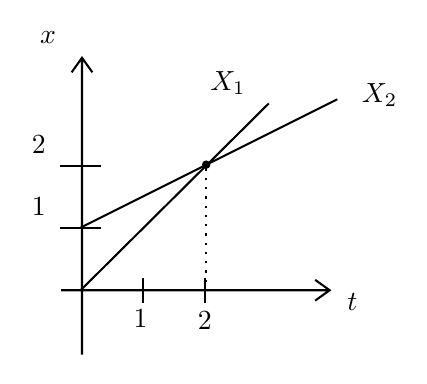
\begin{tikzpicture}[x=0.75pt,y=0.75pt,yscale=-1,xscale=1]
            %uncomment if require: \path (0,300); %set diagram left start at 0, and has height of 300

            %Shape: Axis 2D [id:dp3242275334401292] 
            \draw  (230.67,150) -- (360,150)(240.67,38) -- (240.67,181) (353,145) -- (360,150) -- (353,155) (235.67,45) -- (240.67,38) -- (245.67,45)  ;
            %Straight Lines [id:da6800909913200827] 
            \draw    (270,144) -- (270,156) ;
            %Straight Lines [id:da504363558290425] 
            \draw    (300,144) -- (300,156) ;
            %Straight Lines [id:da41768238504122124] 
            \draw  [dash pattern={on 0.84pt off 2.51pt}]  (300.5,150.5) -- (300.5,89.5) ;
            %Shape: Circle [id:dp23983039955771324] 
            \draw  [fill={rgb, 255:red, 47; green, 0; blue, 0 }  ,fill opacity=1 ] (299,89.5) .. controls (299,88.67) and (299.67,88) .. (300.5,88) .. controls (301.33,88) and (302,88.67) .. (302,89.5) .. controls (302,90.33) and (301.33,91) .. (300.5,91) .. controls (299.67,91) and (299,90.33) .. (299,89.5) -- cycle ;
            %Straight Lines [id:da8200181075779964] 
            \draw    (240,150) -- (330.67,60) ;
            %Straight Lines [id:da5662793742139913] 
            \draw    (230,120) -- (250,120) ;
            %Straight Lines [id:da2599786825287116] 
            \draw    (239.67,120) -- (363.67,58) ;
            %Straight Lines [id:da18823594983513814] 
            \draw    (230,90) -- (250,90) ;

            % Text Node
            \draw (264,158) node [anchor=north west][inner sep=0.75pt]   [align=left] {$\displaystyle 1$};
            % Text Node
            \draw (219,24) node [anchor=north west][inner sep=0.75pt]   [align=left] {$\displaystyle x$};
            % Text Node
            \draw (301,43) node [anchor=north west][inner sep=0.75pt]   [align=left] {$\displaystyle X_{1}$};
            % Text Node
            \draw (215,104) node [anchor=north west][inner sep=0.75pt]   [align=left] {$\displaystyle 1$};
            % Text Node
            \draw (374,49) node [anchor=north west][inner sep=0.75pt]   [align=left] {$\displaystyle X_{2}$};
            % Text Node
            \draw (295,159) node [anchor=north west][inner sep=0.75pt]   [align=left] {$\displaystyle 2$};
            % Text Node
            \draw (367,150) node [anchor=north west][inner sep=0.75pt]   [align=left] {$\displaystyle t$};
            % Text Node
            \draw (215,74) node [anchor=north west][inner sep=0.75pt]   [align=left] {$\displaystyle 2$};

            \end{tikzpicture}
        \end{center}
    \end{figure}
    Basta igualar y despejar el tiempo para ver en qué instante chocan. En este caso es claro, pues $t = 1 + t/2 \iff t/2 = 1 \iff t = 2$.
    Esta colisión podría derivar en un absurdo a priori:
    $$1 = u_0(0) \stackrel{(*)}{=} u(2,\overbrace{X_1(2;0,0)}^{X_2(2;0,1)}) = u(2,X_2(2;0,1)) = u_0(1) = 1/2$$
    donde se ha usado en $(*)$ que $X_1$ es una característica y \eqref{eq:ec12}. Todo lo anterior es correcto. La única explicación posible es que 
    la colisión entre características se traduce en la discontinuidad de la solución. Donde las características chocan, la solución salta. Realmente 
    estamos evaluando en un punto donde no podemos evaluar, porque los límites laterales no coinciden, a pesar de que el dato inicial $u(0,x) = 1/(1+x^2) \in C^\infty(\R)$.
\end{ejemplo}

\begin{ejercicio}\label{ejercicio:ej26}
    Fijado en \eqref{eq:ec9} un dato inicial $u_0 \in C^1(\R)$ (marco de la teoría clásica), \underline{decreciente}\footnote{Esta será la condición fundamental para que 
    las características colisionen.} y con derivada inferiormente acotada\footnote{Cuestión técnica.}, comprueba\footnote{Se trata de escribir cuándo se tienen garantías de 
    que las características choquen (en tal caso tendremos garantías también de discontinuidad de la solución). Caracterizar cuál es el primer tiempo de choque de dos características 
    cualesquiera. A partir de ahí se produce el salto de la solución y se pierde la continuidad.} que el primer instante en el que dos rectas características 
    cualesquiera colisionan, denotado por $T^*$, viene dado por $$T^{*} = - \dfrac{1}{\inf_{x \in \R} \{u_0'(x)\}}$$

    Para hacer el ejercicio, lo más sencillo es verlo como una aplicación inmediata del Teorema del Valor Medio. Así sale en dos líneas. Tomar dos características cualquiera,
    que sabemos que son rectas, chocamos (vemos en qué instantes chocan), tomamos mínimos, y ahí se aplica el Teorema del Valor Medio.

    % TODO: Hacer
\end{ejercicio}

De esta manera, la solución de Burgers definida en $u : \left[0, T^{*} \right[ \times \R \to \R$ la solución sería $C^1$, y se podría aplicar la teoría clásica. Aún así,
$T^{*}$ puede ser muy pequeño. \\

% Lo que viene es ejercicio de Parcial 1

Visto todo lo anterior, lo natural parece ser trabajar con soluciones débiles, dado que no nos exigen ni continuidad. Lo que resta de estudio de la ecuación de Burgers, que es poco,
porque no se puede hacer mucho más sin entrar en cosas demasiado complicadas, es estudiar cuáles son las soluciones débiles más sencillas del modelo de Burgers. Estas serán de la forma:
\begin{equation}\label{eq:ec13}
    u(t,x) = \begin{cases}
        u^{-}, \quad& x < \lm t \\
        u^{+}, \quad& x > \lm t
    \end{cases}
\end{equation}

Gráficamente\footnote{Se ha representado con cierto $\lm > 0$.}:

\begin{figure}[H]
    \begin{center}
        \tikzset{every picture/.style={line width=0.75pt}} %set default line width to 0.75pt        

        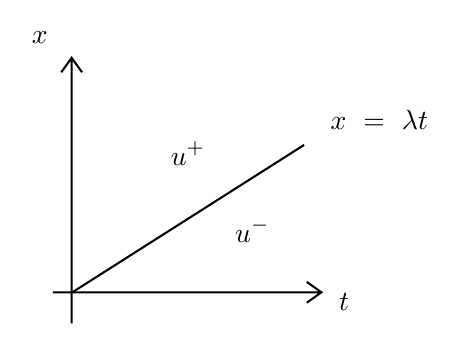
\begin{tikzpicture}[x=0.75pt,y=0.75pt,yscale=-1,xscale=1]
        %uncomment if require: \path (0,300); %set diagram left start at 0, and has height of 300

        %Shape: Axis 2D [id:dp3242275334401292] 
        \draw  (230.67,151) -- (360,151)(239.67,38) -- (239.67,166) (353,146) -- (360,151) -- (353,156) (234.67,45) -- (239.67,38) -- (244.67,45)  ;
        %Straight Lines [id:da8200181075779964] 
        \draw    (240,151) -- (351.67,80) ;

        % Text Node
        \draw (219,24) node [anchor=north west][inner sep=0.75pt]   [align=left] {$\displaystyle x$};
        % Text Node
        \draw (363,62) node [anchor=north west][inner sep=0.75pt]   [align=left] {$\displaystyle x\ =\ \lambda t$};
        % Text Node
        \draw (367,150) node [anchor=north west][inner sep=0.75pt]   [align=left] {$\displaystyle t$};
        % Text Node
        \draw (317,114) node [anchor=north west][inner sep=0.75pt]   [align=left] {$\displaystyle u^{-}$};
        % Text Node
        \draw (286,77) node [anchor=north west][inner sep=0.75pt]   [align=left] {$\displaystyle u^{+}$};


        \end{tikzpicture}
    \end{center}
\end{figure}

Las soluciones tendrán lado constante a la izquierda de $x = \lm t$ y a la derecha. Para trabajar con estas soluciones, el dato inicial del que hay que partir debe ser 

\begin{equation}\label{eq:ec14}
    u_0(x) = \begin{cases}
        u^{-}, \quad& x < 0 \\
        u^{+}, \quad& x > 0
    \end{cases}
\end{equation}


Cuando a la ecuación de Burgers se le asocia un dato inicial con salto ($u^{-}$ por arriba y $u^{+}$ por abajo). Este tipo de dato inicial da pie al siguiente tipo más específico de problema, conocido como \underline{problema de Riemann}:
\begin{definicion}[Problema de Riemann]\label{definicion:d21}
    El problema de Burgers \eqref{eq:ec9} con un dato inicial de la forma \eqref{eq:ec14} se denomina problema de Riemann. \\
\end{definicion}

%\begin{observacion}
%    Lo que hace el modelo de Burgers es ``inclinar'' la recta $x=0$ a $x=\lm t$. \\
%\end{observacion}
% El único valor posible de $\lm = \dfrac{1}{2}(u^{+} + u^{-})$ para que $u$ sea solución débil.
% Veremos el martes bajo qué condiciones esto es un problema de Riemann
% Quizá sugiera que el que entregue el ejercicio propuesto lo cuente como participación.
% Seguramente usaremos el lunes 19 para terminar el bloque, y recomienda llevarse la prueba a la semana siguiente o más. Lo mejor sería retrasarla al menos una semana dice. 
% 13.10.2026
Retomamos el problema \eqref{eq:ec9}. Una solución débil de este problema era \eqref{eq:ec13}, donde $u^{-}, u^{+}, \lm \in \R$, para cierto $\lm$, y el dato inicial era \eqref{eq:ec14}.
Así, el modelo lo que hace es transformar la recta $x=0$ (inicial) en la recta $x = \lm t$, y se mantienen los valores 
originales $u^{-}$ y $u^{+}$. \\

Queremos ver entonces cuándo \eqref{eq:ec13} es solución de \eqref{eq:ec9}, cuando tenemos un dato inicial de la forma \eqref{eq:ec14}. \\

El siguiente resultado será de gran utilidad:

\begin{teo}[Condición de salto de Rankine-Hugoniot]\label{teo:t2}
    Sean\footnote{Se impone que $u^{+} \neq u^{-}$ para que exista un salto. En otro caso la función es constante y no hay salto.} $\lm, u^{+}, u^{-} \in \R$ : $u^{+} \neq u^{-}$. Entonces la función \eqref{eq:ec13} es una solución débil del problema de Riemann asociado a \eqref{eq:ec9}
    si y solamente si $$\lm = \dfrac{\dfrac{1}{2}(u^{+})^2 - \dfrac{1}{2}(u^{-})^2}{u^{+} - u^{-}} = \dfrac{1}{2}(u^{+} + u^{-})$$ 
\end{teo}

\begin{observacion}
    El significado físico de $\lm$ es la velocidad a la que varía la recta. Geométricamente sería la pendiente. Aunque lo vamos a utilizar para 
    Burgers, el Teorema \ref{teo:t2} vale para cualquier modelo no lineal:
    \begin{equation}
        \begin{cases}
            \dfrac{\partial u}{\partial t} + \dfrac{\partial}{\partial x}(f(u)) = 0 \\
            u(0,x) = u_0(x)
        \end{cases}
    \end{equation}
    y en tal caso el valor de $\lm$ es:
    $$\lm = \dfrac{f(u^{+}) - f(u^{-})}{u^{+} - u^{-}}$$
\end{observacion}

Antes de demostrar el Teorema \ref{teo:t2}, veamos qué significa ser solución débil del problema de Burgers \eqref{eq:ec9}:

\begin{definicion}[Solución débil de \eqref{eq:ec9}]
    Buscamos una función $u \in L_{loc}^1(\left[0, T\right[ \times \R)$ tal que
    $$\int_{0}^{T} \int_{-\infty}^{+\infty} \left( \dfrac{\partial u}{\partial t} + \dfrac{\partial}{\partial x} \left( \dfrac{u^2}{2} \right) \right) \varphi \,dx\,dt = 0$$
    Integrando por partes:
    $$\int_{-\infty}^{+\infty} u(0,x) \varphi(0,x)\,dx + \int_{0}^{T} \int_{-\infty}^{+\infty} u \dfrac{\partial \varphi}{\partial t}\,dx\,dt
    + \int_{0}^{T} \int_{-\infty}^{+\infty} \dfrac{u^2}{2} \dfrac{\partial \varphi}{\partial x}\,dx\,dt = 0$$
    Así pues, si $u \in L_{loc}^1(\left[0, T\right[ \times \R)$, entonces 
    \begin{equation}\label{eq:ec15}
        \boxed{\int_{0}^{T} \int_{-\infty}^{+\infty} \left[ u \dfrac{\partial \varphi}{\partial t} + \dfrac{u^2}{2} \dfrac{\partial \varphi}{\partial x} \right]\,dx\,dt = - 
        \int_{-\infty}^{+\infty} u_0(x) \varphi(0,x)\,dx}
    \end{equation}
    para toda $\varphi \in C_c^1(\left[0, T\right[ \times \R)$.
\end{definicion}

Recordamos para la demostración del Teorema \ref{teo:t2} el Teorema de la Divergencia\footnote{También conocido como Teorema de Gauss.}:

\begin{teo}[de la Divergencia]
    Sea $\Omega \subset \R^N$ un abierto cuya frontera $\partial \Omega$ es de clase $C^1$, y sea $A \in C^1(\bar{\Omega}, \R^N)$ un campo vectorial.
    Entonces
    $$\int_{\Omega} \di(A)\,dx = \int_{\partial \Omega} A \cdot \vec{\eta} \, d \sigma$$
    donde $\vec{\eta}$ es el vector normal unitario exterior a $\partial \Omega$.
\end{teo}

\begin{proof}
    La función \eqref{eq:ec13} cumple \eqref{eq:ec15} si 
    \begin{equation}\label{eq:ec16}
        \begin{aligned}
            &\overbrace{\int_{0}^{T} \int_{-\infty}^{\lm t}
            \left[ u^{-} \dfrac{\partial \varphi}{\partial t}
            + \dfrac{(u^{-})^2}{2}
            \dfrac{\partial \varphi}{\partial x} \right]
            \,dx\,dt}^{I_1} \\
            &+ \overbrace{\int_{0}^{T} \int_{\lm t}^{+\infty}
            \left[ u^{+} \dfrac{\partial \varphi}{\partial t}
            + \dfrac{(u^{+})^2}{2}
            \dfrac{\partial \varphi}{\partial x} \right]
            \,dx\,dt}^{I_2} = \\
            &- \int_{-\infty}^{0} u^{-}\varphi(0,x)\,dx
            - \int_{0}^{+\infty} u^{+}\varphi(0,x)\,dx
        \end{aligned}
    \end{equation}
    Para ver esto solo hay que aplicar el Teorema de la Divergencia y sale directamente. Consideramos 
    $$A^{\mp} = \left(u^{\mp} \varphi, \dfrac{(u^{\mp})^2}{2} \varphi \right)$$
    y $$\di_{(t,x)}(A^{\mp}) = \dfrac{\partial u^{\mp} \varphi}{\partial t} + \dfrac{\partial}{\partial x} \left( \dfrac{(u^{\mp})^2}{2} \varphi \right) = $$
    $$u^{\mp} \dfrac{\partial \varphi}{\partial t} + \dfrac{(u^{\mp})^2}{2} \dfrac{\partial \varphi}{\partial x}$$
    El resultado de aplicar el Teorema de la Divergencia es:
    $$I_1 = - \int_{-\infty}^{0} u^{-} \varphi(0,x) \,dx - \int_{0}^{T} \varphi(t, \lm t) \left( \lm u^{-} - \dfrac{(u^{-})^2}{2} \right)$$
    $$I_2 = - \int_{0}^{+\infty} u^{+} \varphi(0,x) \,dx + \int_{0}^{T} \varphi(t, \lm t) \left( \lm u^{+} - \dfrac{(u^{+})^2}{2} \right)$$
    Si sustituimos en \eqref{eq:ec16} el resultado obtenido en $I_1$ e $I_2$, nos queda:
    $$\int_{0}^{T} \varphi(t,\lm t) \left( \lm u^{+} - \dfrac{(u^+)^2}{2} - \lm u^{-} + \dfrac{(u^-)^2}{2} \right) \, dt = 0$$
    para toda función $\varphi$ test, por lo que la única alternativa es que, al igualar a $0$ el otro factor del integrando, y despejando $\lm$, resulta que:
    $$\lm = \dfrac{\dfrac{1}{2}(u^{+})^2 - \dfrac{1}{2}(u^{-})^2}{u^{+} - u^{-}} = \dfrac{1}{2}(u^{+} + u^{-})$$
    como se quería demostrar\footnote{Al final hemos aplicado la versión débil del lema fundamental del cálculo de variaciones.}.
\end{proof}

\begin{ejercicio} % TODO: Hacer
    Comprobar que en efecto salen esos valores de $I_1$ e $I_2$ tras aplicar el Teorema de la Divergencia.
\end{ejercicio}

\begin{observacion}
    Si consideramos $$A^{-} = \left(u^{-} \varphi, \dfrac{(u^-)^2}{2} \varphi \right)$$ y
    $$\Omega = \left[0, T \right[ \times \left]-\infty, \lm t \right[$$
    Gráficamente:
    \begin{figure}[H]
        \begin{center}
            \tikzset{every picture/.style={line width=0.75pt}} %set default line width to 0.75pt        

            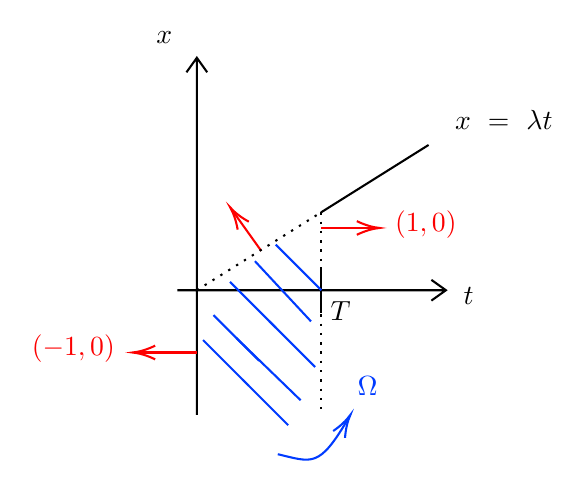
\begin{tikzpicture}[x=0.75pt,y=0.75pt,yscale=-1,xscale=1]
            %uncomment if require: \path (0,300); %set diagram left start at 0, and has height of 300

            %Shape: Axis 2D [id:dp3242275334401292] 
            \draw  (230.67,150) -- (360,150)(240,38) -- (240,210) (353,145) -- (360,150) -- (353,155) (235,45) -- (240,38) -- (245,45)  ;
            %Straight Lines [id:da8200181075779964] 
            \draw    (299.83,112.5) -- (351.67,80) ;
            %Straight Lines [id:da10207814113213398] 
            \draw    (300,139) -- (300,161) ;
            %Straight Lines [id:da4016638819857854] 
            \draw  [dash pattern={on 0.84pt off 2.51pt}]  (299.83,112.5) -- (299.83,210.5) ;
            %Straight Lines [id:da7811408021976621] 
            \draw [color={rgb, 255:red, 0; green, 59; blue, 255 }  ,draw opacity=1 ]   (278,128) -- (300,150) ;
            %Straight Lines [id:da45167587101332696] 
            \draw [color={rgb, 255:red, 0; green, 59; blue, 255 }  ,draw opacity=1 ]   (268,136) -- (295,165) ;
            %Straight Lines [id:da8532721754574758] 
            \draw [color={rgb, 255:red, 0; green, 59; blue, 255 }  ,draw opacity=1 ]   (256,146) -- (278,168) ;
            %Straight Lines [id:da21649060037233314] 
            \draw [color={rgb, 255:red, 0; green, 59; blue, 255 }  ,draw opacity=1 ]   (275,165) -- (297,187) ;
            %Straight Lines [id:da7942393059803331] 
            \draw [color={rgb, 255:red, 0; green, 59; blue, 255 }  ,draw opacity=1 ]   (248,162) -- (270,184) ;
            %Straight Lines [id:da6329598689513399] 
            \draw [color={rgb, 255:red, 0; green, 59; blue, 255 }  ,draw opacity=1 ]   (259,173) -- (290,203) ;
            %Straight Lines [id:da5635607272548492] 
            \draw [color={rgb, 255:red, 0; green, 59; blue, 255 }  ,draw opacity=1 ]   (243,174) -- (265,196) ;
            %Straight Lines [id:da6741985877594474] 
            \draw [color={rgb, 255:red, 0; green, 59; blue, 255 }  ,draw opacity=1 ]   (262,193) -- (284,215) ;
            %Curve Lines [id:da5966350701002826] 
            \draw [color={rgb, 255:red, 0; green, 59; blue, 255 }  ,draw opacity=1 ]   (279,229) .. controls (295.66,232.92) and (298.87,235.88) .. (313.11,211.53) ;
            \draw [shift={(314,210)}, rotate = 119.98] [color={rgb, 255:red, 0; green, 59; blue, 255 }  ,draw opacity=1 ][line width=0.75]    (10.93,-3.29) .. controls (6.95,-1.4) and (3.31,-0.3) .. (0,0) .. controls (3.31,0.3) and (6.95,1.4) .. (10.93,3.29)   ;
            %Straight Lines [id:da4584837957354798] 
            \draw [color={rgb, 255:red, 253; green, 0; blue, 0 }  ,draw opacity=1 ]   (240,180) -- (211,180) ;
            \draw [shift={(209,180)}, rotate = 360] [color={rgb, 255:red, 253; green, 0; blue, 0 }  ,draw opacity=1 ][line width=0.75]    (10.93,-3.29) .. controls (6.95,-1.4) and (3.31,-0.3) .. (0,0) .. controls (3.31,0.3) and (6.95,1.4) .. (10.93,3.29)   ;
            %Straight Lines [id:da24433253893145346] 
            \draw [color={rgb, 255:red, 253; green, 0; blue, 0 }  ,draw opacity=1 ]   (300,120) -- (326,120) ;
            \draw [shift={(328,120)}, rotate = 180] [color={rgb, 255:red, 253; green, 0; blue, 0 }  ,draw opacity=1 ][line width=0.75]    (10.93,-3.29) .. controls (6.95,-1.4) and (3.31,-0.3) .. (0,0) .. controls (3.31,0.3) and (6.95,1.4) .. (10.93,3.29)   ;
            %Straight Lines [id:da8693895743082151] 
            \draw [color={rgb, 255:red, 253; green, 0; blue, 0 }  ,draw opacity=1 ]   (271,131) -- (257.16,111.63) ;
            \draw [shift={(256,110)}, rotate = 54.46] [color={rgb, 255:red, 253; green, 0; blue, 0 }  ,draw opacity=1 ][line width=0.75]    (10.93,-3.29) .. controls (6.95,-1.4) and (3.31,-0.3) .. (0,0) .. controls (3.31,0.3) and (6.95,1.4) .. (10.93,3.29)   ;
            %Straight Lines [id:da002150546491489602] 
            \draw  [dash pattern={on 0.84pt off 2.51pt}]  (240,150) -- (299.83,112.5) ;

            % Text Node
            \draw (219,24) node [anchor=north west][inner sep=0.75pt]   [align=left] {$\displaystyle x$};
            % Text Node
            \draw (363,62) node [anchor=north west][inner sep=0.75pt]   [align=left] {$\displaystyle x\ =\ \lambda t$};
            % Text Node
            \draw (367,147) node [anchor=north west][inner sep=0.75pt]   [align=left] {$\displaystyle t$};
            % Text Node
            \draw (303,154) node [anchor=north west][inner sep=0.75pt]   [align=left] {$\displaystyle T$};
            % Text Node
            \draw (316,190) node [anchor=north west][inner sep=0.75pt]   [align=left] {$\displaystyle \textcolor[rgb]{0,0.23,1}{\Omega }$};
            % Text Node
            \draw (159,170) node [anchor=north west][inner sep=0.75pt]   [align=left] {$\displaystyle \textcolor[rgb]{0.99,0,0}{( -1,0)}$};
            % Text Node
            \draw (334,110) node [anchor=north west][inner sep=0.75pt]   [align=left] {$\displaystyle \textcolor[rgb]{0.99,0,0}{(}\textcolor[rgb]{0.99,0,0}{1,0}\textcolor[rgb]{0.99,0,0}{)}$};


            \end{tikzpicture}
        \end{center}
    \end{figure}
\end{observacion}
% Mañana vemos los dos tipos específicos de soluciones de la ecuación de Burgers, que son las ondas de choque, y las ondas de rarefacción.
% El lunes o martes será la última clase, seguro. En principio el lunes se resuelven los ejercicios y terminaríamos el bloque. Ya empezaría
% La parte siguiente.
El choque en las trayectorias características se traduce en un salto en la solución. \\

También se comentó al principio el problema de la no unicidad. Veamos el siguiente ejemplo:
\begin{ejemplo}
    Consideramos el siguiente dato inicial para el problema de Riemann:
    \begin{equation*}
        u_0(x) = \begin{cases}
            1 \quad& x<0 \\
            0 \quad& x>0
        \end{cases}
    \end{equation*}
    Por el Teorema \ref{teo:t2}, la solución es 
    \begin{equation*}
        u(t,x) = \begin{cases}
            1 \quad& x < \lm t \\
            0 \quad& x > \lm t
        \end{cases}
    \end{equation*}
    Para $\lm = 1/2$ (valor dado por la condición de salto de Rankine-Hugoniot). Este tipo de soluciones se denominan \underline{ondas de choque}.
    Aquí el dato inicial era decreciente y sabemos entonces que las trayectorias características se van a encontrar.
\end{ejemplo}

\begin{observacion}
    Si la función tuviera más trozos, habría que comparar los trozos dos a dos, pero el teorema seguiría siendo válido. Veremos un ejemplo con tres trozos.
    Lo importante es que sea \textbf{constante a trozos}. \\

    Además, si el dato inicial fuera de la forma 
    $$u_0(x) = \begin{cases}
        u^{-} \quad& x < a \\
        u^{+} \quad& x > a
    \end{cases}$$
    para cualquier $a \in \R$, se podría considerar el cambio de variable $y = x-a$, aplicar el Teorema \ref{teo:t2}, y deshacer el cambio, por 
    lo que sigue siendo válido para traslaciones de la abscisa en la que se produce el salto en el dato inicial. 
\end{observacion}

\begin{ejemplo}
    En este caso, consideramos el dato inicial \underline{creciente}
    \begin{equation*}
        u_0(x) = \begin{cases}
            0 \quad& x < 0 \\
            1 \quad& x > 0
        \end{cases}
    \end{equation*}
    Nuevamente, por el Teorema \ref{teo:t2}, la solución es 
    \begin{equation*}
        u(t,x) = \begin{cases}
            0 \quad& x < t/2 \\
            1 \quad& x > t/2
        \end{cases}
    \end{equation*}
    En este caso, tenemos infinitas soluciones, ya que, para cada $\alpha \in \left]0, 1 \right[$, tenemos las siguientes soluciones (ondas de choque también):
    \begin{equation*}
        u_\alpha(t,x) = \begin{cases}
            0 \quad& x < \frac{\alpha t}{2} \\
            \alpha \quad& \frac{\alpha t}{2} < x < \frac{(\alpha+1) t}{2} \\
            1 \quad& x > \frac{(\alpha+1) t}{2} \\
        \end{cases}
    \end{equation*}
    Pero vamos más allá. Este problema tiene más soluciones, de una naturaleza \textbf{completamente distinta} a las ondas de choque. Una de estas
    soluciones nuevas es:
    \begin{equation}\label{eq:ec18}
        u(t,x) = \begin{cases}
            0 \quad& x < 0 \\
            \frac{x}{t} \quad& 0 \leq x \leq t \\
            1 \quad& x > t
        \end{cases}
    \end{equation}
    Esta solución es destacable porque es \textbf{continua}. Esto se debe a que el dato inicial es \textbf{creciente}\footnote{Si fuera
    decreciente, sabemos que las características chocan y se pierde la continuidad.}.
    En términos de las trayectorias características de la ecuación de Burgers (que, recordemos, son rectas con origen el punto de arranque 
    y pendiente el dato inicial, de la forma \eqref{eq:ec17}). Gráficamente\footnote{Se han intercambiado los ejes para ver con más claridad el lugar que ocupan las ondas de rarefacción.}:
    \begin{figure}[H]
        \begin{center}
            \tikzset{every picture/.style={line width=0.75pt}} %set default line width to 0.75pt        

            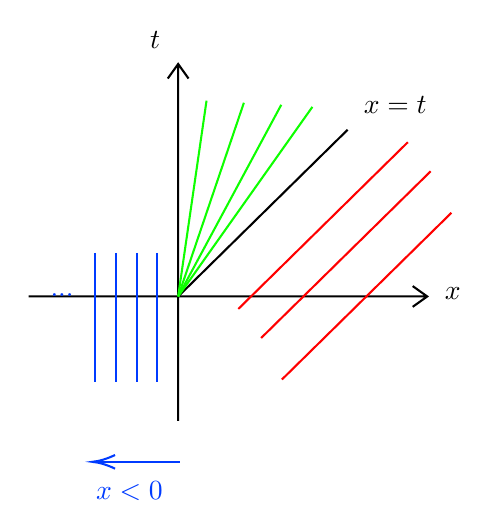
\begin{tikzpicture}[x=0.75pt,y=0.75pt,yscale=-1,xscale=1]
            %uncomment if require: \path (0,300); %set diagram left start at 0, and has height of 300

            %Shape: Axis 2D [id:dp3242275334401292] 
            \draw  (168,150) -- (360,150)(240,38) -- (240,210) (353,145) -- (360,150) -- (353,155) (235,45) -- (240,38) -- (245,45)  ;
            %Straight Lines [id:da8200181075779964] 
            \draw    (240,150) -- (321.67,69.67) ;
            %Straight Lines [id:da7811408021976621] 
            \draw [color={rgb, 255:red, 0; green, 59; blue, 255 }  ,draw opacity=1 ]   (230,129) -- (230,191) ;
            %Straight Lines [id:da9902153940282713] 
            \draw [color={rgb, 255:red, 0; green, 59; blue, 255 }  ,draw opacity=1 ]   (220,129) -- (220,191) ;
            %Straight Lines [id:da46681775109807866] 
            \draw [color={rgb, 255:red, 0; green, 59; blue, 255 }  ,draw opacity=1 ]   (210,129) -- (210,191) ;
            %Straight Lines [id:da2862107334178614] 
            \draw [color={rgb, 255:red, 0; green, 59; blue, 255 }  ,draw opacity=1 ]   (200,129) -- (200,191) ;
            %Straight Lines [id:da891584242145164] 
            \draw [color={rgb, 255:red, 0; green, 59; blue, 255 }  ,draw opacity=1 ]   (240.67,229.67) -- (200.67,229.67) ;
            \draw [shift={(198.67,229.67)}, rotate = 360] [color={rgb, 255:red, 0; green, 59; blue, 255 }  ,draw opacity=1 ][line width=0.75]    (10.93,-3.29) .. controls (6.95,-1.4) and (3.31,-0.3) .. (0,0) .. controls (3.31,0.3) and (6.95,1.4) .. (10.93,3.29)   ;
            %Straight Lines [id:da02222492658014852] 
            \draw [color={rgb, 255:red, 255; green, 0; blue, 0 }  ,draw opacity=1 ]   (280,170) -- (361.67,89.67) ;
            %Straight Lines [id:da4338095240978027] 
            \draw [color={rgb, 255:red, 255; green, 0; blue, 0 }  ,draw opacity=1 ]   (290,190) -- (371.67,109.67) ;
            %Straight Lines [id:da7151116176791149] 
            \draw [color={rgb, 255:red, 255; green, 0; blue, 0 }  ,draw opacity=1 ]   (269,156) -- (350.67,75.67) ;
            %Straight Lines [id:da012982910756638821] 
            \draw [color={rgb, 255:red, 14; green, 255; blue, 0 }  ,draw opacity=1 ]   (240,150) -- (304.67,58.67) ;
            %Straight Lines [id:da44861127255647437] 
            \draw [color={rgb, 255:red, 14; green, 255; blue, 0 }  ,draw opacity=1 ]   (240,150) -- (289.67,57.67) ;
            %Straight Lines [id:da9915204219627409] 
            \draw [color={rgb, 255:red, 14; green, 255; blue, 0 }  ,draw opacity=1 ]   (240,150) -- (271.67,56.67) ;
            %Straight Lines [id:da1270037446521043] 
            \draw [color={rgb, 255:red, 14; green, 255; blue, 0 }  ,draw opacity=1 ]   (240,150) -- (253.67,55.67) ;

            % Text Node
            \draw (367,144) node [anchor=north west][inner sep=0.75pt]   [align=left] {$\displaystyle x$};
            % Text Node
            \draw (328,52) node [anchor=north west][inner sep=0.75pt]   [align=left] {$\displaystyle x=t$};
            % Text Node
            \draw (225,21) node [anchor=north west][inner sep=0.75pt]   [align=left] {$\displaystyle t$};
            % Text Node
            \draw (177,147) node [anchor=north west][inner sep=0.75pt]   [align=left] {\textcolor[rgb]{0,0.23,1}{...}};
            % Text Node
            \draw (199,237.67) node [anchor=north west][inner sep=0.75pt]   [align=left] {$\displaystyle \textcolor[rgb]{0,0.23,1}{x< 0}$};


            \end{tikzpicture}
        \end{center}
    \end{figure}
    donde se muestran las siguientes trayectorias características: 
    \begin{equation*}
        X(t;0,x) = \begin{cases}
            x \quad& x < 0 \\
            x + t \quad& x > 0
        \end{cases}
    \end{equation*}
\end{ejemplo}

Como podemos ver, las trayectorias características dejan un hueco entre $x=0$ y $x=t$. Las rectas verdes con las que se rellena este hueco 
dan pie a la siguiente definición: 

\begin{definicion}[Ondas de Rarefacción]
    Las soluciones al problema de Riemann (\ref{definicion:d21}) de la forma \eqref{eq:ec18} se denominan \underline{ondas de rarefacción}. 
    Nuevamente, es importante recalcar que solo es posible encontrar este tipo de soluciones cuando el dato inicial es \underline{creciente}.
\end{definicion}

\begin{observacion}
    Si cambiamos de escala, es decir, pasamos de $(t,x) \mapsto (\alpha t, \alpha x)$, para cierto $\alpha \in \R$, la solución sigue siendo válida.
    En efecto, tenemos que 
    $$u(t,x) = U \left( \dfrac{x}{t} \right) \rightsquigarrow 
    U'\left( \dfrac{x}{t} \right) \left( - \dfrac{x}{t^2} \right) + U \left( \dfrac{x}{t} \right) U' \left( \dfrac{x}{t} \right) \dfrac{1}{t} = 0$$
    $$U' \left( \dfrac{x}{t} \right) \neq 0 \Longrightarrow - \dfrac{x}{t^2} + U \left( \dfrac{x}{t} \right) \dfrac{1}{t} = 0 \iff$$
    \begin{equation}\label{eq:ec19}
        U \left( \dfrac{x}{t} \right) = \dfrac{x}{t}
    \end{equation}
    Esta última se conoce como solución \underline{autosemejante} o \underline{autosimilar}. Es la que ``rellena el hueco'' que dejan las ondas 
    de rarefacción.
\end{observacion}

\begin{observacion}
    Algunas conclusiones:
    \begin{itemize}
        \item Si el modelo de transporte no podemos aspirar a recuperar las propiedades ``buenas''.
        \item No podemos decir que el problema esté bien planteado en el sentido de la existencia y unicidad.
        \item Es relevante la monotonía del dato inicial.
        \begin{itemize}
            \item Si es decreciente, las características se encontrarán y tendremos un salto.
            \item Si es creciente, aparte de las ondas de choque, podemos encontrar perfiles autosimilares del tipo \eqref{eq:ec19}, generando 
            ondas de rarefacción.
        \end{itemize}
    \end{itemize}
\end{observacion}

Algunos ejercicios para concluir el bloque:

\begin{ejercicio}
    Resolver los siguientes problemas (la ecuación es la de Burgers siempre, y solo cambia el dato inicial):
    $$\dfrac{\partial u}{\partial t} + u \dfrac{\partial u}{\partial x} = 0$$
    para los siguientes datos iniciales, y escribir cómo son las trayectorias características:
    \begin{itemize}
        \item $u_0(x) = \begin{cases}
            2 \quad& x < 0 \\
            1 \quad& 0 < x < 2 \\
            0 \quad& x < 2
        \end{cases}$. \\

        En primer lugar obtenemos las trayectorias características:
        $$X(t; 0, x) = x + u_0(x) t = \begin{cases}
            x + 2t \quad& x < 0 \\
            x + t \quad& 0 < x < 2 \\
            x \quad& x > 2
        \end{cases}$$
        Gráficamente\footnote{El dibujo siempre ayuda en estos casos.}:
        \begin{figure}[H]
            \begin{center}
                \tikzset{every picture/.style={line width=0.75pt}} %set default line width to 0.75pt        
                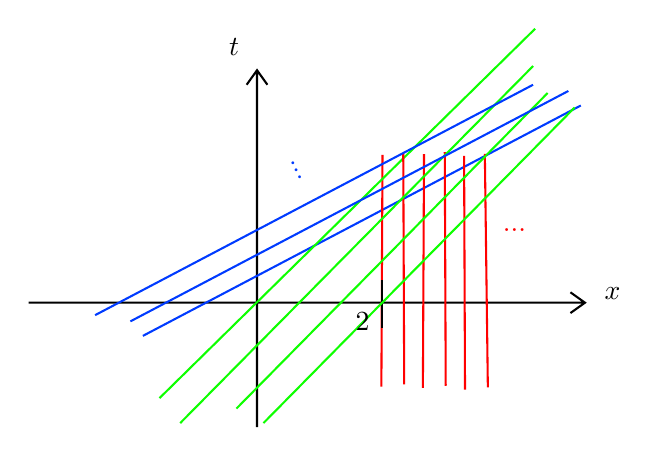
\begin{tikzpicture}[x=0.75pt,y=0.75pt,yscale=-1,xscale=1]
                    %uncomment if require: \path (0,300); %set diagram left start at 0, and has height of 300

                    %Shape: Axis 2D [id:dp3242275334401292] 
                    \draw  (130,150) -- (398,150)(240,38) -- (240,210) (391,145) -- (398,150) -- (391,155) (235,45) -- (240,38) -- (245,45)  ;
                    %Straight Lines [id:da2862107334178614] 
                    \draw [color={rgb, 255:red, 0; green, 59; blue, 255 }  ,draw opacity=1 ]   (396,55) -- (185,166) ;
                    %Straight Lines [id:da02222492658014852] 
                    \draw [color={rgb, 255:red, 255; green, 0; blue, 0 }  ,draw opacity=1 ]   (319.91,191.02) -- (320.46,78.46) ;
                    %Straight Lines [id:da4338095240978027] 
                    \draw [color={rgb, 255:red, 255; green, 0; blue, 0 }  ,draw opacity=1 ]   (340.21,191.83) -- (339.76,79.27) ;
                    %Straight Lines [id:da7151116176791149] 
                    \draw [color={rgb, 255:red, 255; green, 0; blue, 0 }  ,draw opacity=1 ]   (299.91,190.39) -- (300.45,78.84) ;
                    %Straight Lines [id:da012982910756638821] 
                    \draw [color={rgb, 255:red, 14; green, 255; blue, 0 }  ,draw opacity=1 ]   (193,196) -- (374,18) ;
                    %Straight Lines [id:da8509471356906648] 
                    \draw    (300,139) -- (300,162) ;
                    %Straight Lines [id:da3794350886499228] 
                    \draw [color={rgb, 255:red, 255; green, 0; blue, 0 }  ,draw opacity=1 ]   (330.91,190.02) -- (330.46,77.46) ;
                    %Straight Lines [id:da6561401855095113] 
                    \draw [color={rgb, 255:red, 255; green, 0; blue, 0 }  ,draw opacity=1 ]   (351.21,190.83) -- (349.76,78.27) ;
                    %Straight Lines [id:da27040052523613545] 
                    \draw [color={rgb, 255:red, 255; green, 0; blue, 0 }  ,draw opacity=1 ]   (310.91,189.39) -- (310.45,77.84) ;
                    %Straight Lines [id:da3632659939494831] 
                    \draw [color={rgb, 255:red, 14; green, 255; blue, 0 }  ,draw opacity=1 ]   (203,208) -- (373,36) ;
                    %Straight Lines [id:da97824068996717] 
                    \draw [color={rgb, 255:red, 14; green, 255; blue, 0 }  ,draw opacity=1 ]   (243.1,208) -- (393,56) ;
                    %Straight Lines [id:da12914183632548215] 
                    \draw [color={rgb, 255:red, 14; green, 255; blue, 0 }  ,draw opacity=1 ]   (230.1,201) -- (380,49) ;
                    %Straight Lines [id:da5712018545643891] 
                    \draw [color={rgb, 255:red, 0; green, 59; blue, 255 }  ,draw opacity=1 ]   (390,48) -- (179,159) ;
                    %Straight Lines [id:da8348964328891428] 
                    \draw [color={rgb, 255:red, 0; green, 59; blue, 255 }  ,draw opacity=1 ]   (373,45) -- (162,156) ;

                    % Text Node
                    \draw (406,141) node [anchor=north west][inner sep=0.75pt]   [align=left] {$\displaystyle x$};
                    % Text Node
                    \draw (225,21) node [anchor=north west][inner sep=0.75pt]   [align=left] {$\displaystyle t$};
                    % Text Node
                    \draw (286,153.5) node [anchor=north west][inner sep=0.75pt]   [align=left] {$\displaystyle 2$};
                    % Text Node
                    \draw (357,113) node [anchor=north west][inner sep=0.75pt]   [align=left] {\textcolor[rgb]{1,0,0}{...}};
                    % Text Node
                    \draw (257.69,78.97) node [anchor=north west][inner sep=0.75pt]  [rotate=-63.09] [align=left] {\textcolor[rgb]{0,0.23,1}{...}};

                \end{tikzpicture}
            \end{center}
        \end{figure}
        Distinguimos dos a dos: el primer dato inicial que consideramos es 
        $$u_1(0,x) = \begin{cases}
            2 \quad& x < 0 \\
            1 \quad& 0 < x < 2
        \end{cases}$$
        Y aplicando la condición de salto de Rankine-Hugoniot (Teorema \ref{teo:t2}) obtenemos que 
        $$\lm = \dfrac{1}{2}(u_1^{+} + u_1^{-}) = \dfrac{3}{2}$$
        Por lo que una primera solución sería 
        $$u_1(t,x) = \begin{cases}
            2 \quad& x < \frac{3t}{2} \\
            1 \quad& x > \frac{3t}{2}
        \end{cases}$$
        Análogamente, el segundo inicial considerado es 
        $$u_2(0,x) = \begin{cases}
            1 \quad& 0 < x < 2 \\
            0 \quad& x > 2
        \end{cases}$$
        Y aplicando la condición de salto de Rankine-Hugoniot (Teorema \ref{teo:t2}) obtenemos que 
        $$\lm = \dfrac{1}{2}(u_2^{+} + u_2^{-}) = \dfrac{1}{2}$$
        Por lo que una segunda solución sería 
        $$u_2(t,x) = \begin{cases}
            1 \quad& x < \frac{t}{2} + 2 \\
            0 \quad& x > \frac{t}{2} + 2
        \end{cases}$$
        En conclusión, la solución conjunta sería 
        $$u(t,x) = \begin{cases}
            2 \quad& x < \frac{3t}{2} \\
            1 \quad& \frac{3t}{2} < x < \frac{t}{2} + 2 \\
            0 \quad& x > \frac{t}{2} + 2
        \end{cases}$$
        Veamos ahora donde corta. Gráficamente:
        \begin{figure}[H]
            \begin{center}
                \tikzset{every picture/.style={line width=0.75pt}} %set default line width to 0.75pt        

                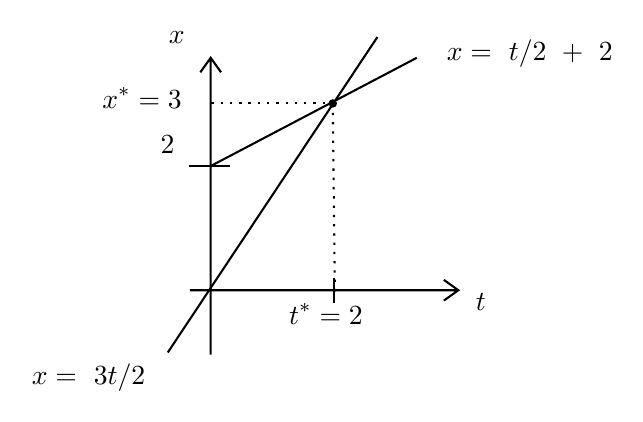
\begin{tikzpicture}[x=0.75pt,y=0.75pt,yscale=-1,xscale=1]
                %uncomment if require: \path (0,300); %set diagram left start at 0, and has height of 300

                %Shape: Axis 2D [id:dp3242275334401292] 
                \draw  (230.67,150) -- (360,150)(240.67,38) -- (240.67,181) (353,145) -- (360,150) -- (353,155) (235.67,45) -- (240.67,38) -- (245.67,45)  ;
                %Straight Lines [id:da504363558290425] 
                \draw    (300,144) -- (300,156) ;
                %Straight Lines [id:da41768238504122124] 
                \draw  [dash pattern={on 0.84pt off 2.51pt}]  (300.5,150.5) -- (299.5,61.5) ;
                %Shape: Circle [id:dp23983039955771324] 
                \draw  [fill={rgb, 255:red, 47; green, 0; blue, 0 }  ,fill opacity=1 ] (298,60) .. controls (298,59.17) and (298.67,58.5) .. (299.5,58.5) .. controls (300.33,58.5) and (301,59.17) .. (301,60) .. controls (301,60.83) and (300.33,61.5) .. (299.5,61.5) .. controls (298.67,61.5) and (298,60.83) .. (298,60) -- cycle ;
                %Straight Lines [id:da8200181075779964] 
                \draw    (220,180) -- (321,28) ;
                %Straight Lines [id:da2599786825287116] 
                \draw    (241,90) -- (340,38) ;
                %Straight Lines [id:da18823594983513814] 
                \draw    (230,90) -- (250,90) ;
                %Straight Lines [id:da9505158034700008] 
                \draw  [dash pattern={on 0.84pt off 2.51pt}]  (241,60) -- (299.5,60) ;

                % Text Node
                \draw (219,24) node [anchor=north west][inner sep=0.75pt]   [align=left] {$\displaystyle x$};
                % Text Node
                \draw (153,184) node [anchor=north west][inner sep=0.75pt]   [align=left] {$\displaystyle x=\ 3t/2$};
                % Text Node
                \draw (277,155) node [anchor=north west][inner sep=0.75pt]   [align=left] {$\displaystyle t^{*} =2$};
                % Text Node
                \draw (367,150) node [anchor=north west][inner sep=0.75pt]   [align=left] {$\displaystyle t$};
                % Text Node
                \draw (215,74) node [anchor=north west][inner sep=0.75pt]   [align=left] {$\displaystyle 2$};
                % Text Node
                \draw (353,28) node [anchor=north west][inner sep=0.75pt]   [align=left] {$\displaystyle x=\ t/2\ +\ 2$};
                % Text Node
                \draw (187,51) node [anchor=north west][inner sep=0.75pt]   [align=left] {$\displaystyle x^{*} =3$};


                \end{tikzpicture}
            \end{center}
        \end{figure}
        Así pues: 
        $$u(2,x) = \begin{cases}
            2 \quad& x < 3 \\
            0 \quad& x > 3
        \end{cases} \stackrel{R.H}{\Longrightarrow} \lm = 1$$
        Si $x = a + \lm t$, evaluando en $(t,x) = (t^*, x^*) = (2,3)$ se tiene que $a = 1$
        y la solución quedaría 
        $$u(t,x) = \begin{cases}
            2 \quad& x < 1 + t \\
            0 \quad& x > 1 + t
        \end{cases}$$
        donde $(t,x) \in \left[2, +\infty \right[ \times \R$.
        \item $u_0(x) = \begin{cases}
            1 \quad& x < -1 \\
            0 \quad& -1 < x < 1 \\
            -1 \quad& x > 1
        \end{cases}$. Este se resuelve análogo al anterior.
        \item $u_0(x) = \begin{cases}
            1 \quad& x < 0 \\
            1-x \quad& 0 \leq x \leq 1 \\
            0 \quad& x > 1
        \end{cases}$. No lo resuelve.
    \end{itemize}
    Para resolver el primer (y segundo) apartado. El primer ``lote'' de trayectorias características chocará con el segundo, y el segundo con el tercero.
    Tendremos dos rectas de discontinuidad distintas. En algún punto ambas rectas chocarán entre sí. Una vez escrita, tendremos un choque con 
    tres tramos que estará bien definido en el sentido de Rankine-Hugoniot hasta el punto en que choquen ambas rectas de discontinuidad.
    Una vez chocan estas dos rectas, al calcularlo veremos que el tramo central de la solución que hemos escrito, colapsa. Así, los tres
    tramos se convierten en dos, también constantes a trozos. Ahí colocamos la nueva condición inicial para saber qué pasa desde el instante de choque
    en adelante. Como ahora el dato inicial solo tiene dos tramos, aplicamos Rankine-Hugoniot una vez. \\

    Como los datos iniciales son decrecientes, no podemos esperar encontrar soluciones continuas. \\

    Para el tercero, que \textbf{no} es un problema de Riemann, porque el dato inicial no es constante a trozos, usamos una propiedad fundamental,
    que es de lo poco que se ``hereda'' del modelo lineal:
    $$\dfrac{d}{dt} (u(t,X(t;0,x))) = 0 \Longrightarrow u(t,X(t;0,x)) = u_0(x)$$
    Lo que se sugiere es aplicar esta propiedad en cada uno de los tramos. En el primero y en el tercero es trivial. La cosa es aplicar en el 
    tramo central a ver qué sale.
\end{ejercicio}

\begin{ejercicio}[Modelos de Tráfico]
    Denotamos $\rho(t,x)$ el número de vehículos por unidad de longitud a lo largo de una carretera en el instante $t$, \textbf{sin contar el propio}.
    Llamamos $u(t,x)$ a la distribución de velocidades de los vehículos. Ténganse además en cuenta las siguientes consideraciones\footnote{Para simplificar el modelo.}:
    \begin{itemize}
        \item Todos los vehículos son del mismo tipo.
        \item Si no hay más vehículos que el propio ($\rho(t,x) = 0$), entonces la velocidad a la que circulo es la máxima posible, pongamos $u = u_{max}$.
        \item Si el número de vehículos es el máximo posible, pongamos $\rho = \rho_{max}$, entonces no nos podemos mover porque la vía está colapsada,
        es decir, $u = 0$.
    \end{itemize}
    En tales circunstancias, el flujo viene descrito por 
    $$f(\rho) = \rho u$$
    Recordemos que en modelos de transporte el flujo era $f(u)$ en:
    \begin{equation}\label{eq:ec20}
        \dfrac{\partial u}{\partial t} + \dfrac{\partial}{\partial x} \left( f(u) \right) = 0
    \end{equation}
    Entonces 
    $$u(\rho) = u_{max} \left( 1 - \dfrac{\rho}{\rho_{max}} \right)$$
    Se pide:
    \begin{enumerate}
        \item Construir el modelo de transporte no lineal para estos datos (es decir, obtener una ecuación de la forma \eqref{eq:ec20}), y verificar que el modelo resultante
        (que será una ecuación lineal que no podemos identificar con nada (lo que nos saldrá no es Burgers, que es el único modelo lineal que no conocemos))
        es reducible a un modelo de Burgers a través del siguiente cambio de variable:
        \begin{equation}\label{eq:ec21}
            R(t,x) = u_{max} - 2 \dfrac{u_{max}}{\rho_{max}} \rho(t,x)
        \end{equation}
        y obtener una ecuación de la forma 
        $$\dfrac{\partial R}{\partial t} + R \dfrac{\partial R}{\partial x} = 0$$
        De esta manera, podemos sacar conclusiones aplicando la teoría conocida de Burgers, y luego volver al modelo original deshaciendo el cambio. \\

        Resolvemos por orden de aparición. Primeramente tenemos que 
        $$\dfrac{\partial \rho}{\partial t} + \dfrac{\partial}{\partial x} f(\rho) = 0$$
        y desarrollando
        $$\dfrac{\partial \rho}{\partial t} + \dfrac{\partial}{\partial x} (\rho u) = 
        \dfrac{\partial \rho}{\partial t} + \dfrac{\partial \rho}{\partial x} u_{max} \left( 1 - \dfrac{\rho}{\rho_{max}} \right) - 
        \rho \dfrac{\partial \rho}{\partial x} \dfrac{u_{max}}{\rho_{max}} =$$
        $$\boxed{\dfrac{\partial \rho}{\partial t} + u_{max} \dfrac{\partial \rho}{\partial x} - 2 \dfrac{u_{max}}{\rho_{max}} \rho \dfrac{\partial \rho}{\partial x} = 0}$$

        Antes de seguir podríamos haber sacado factor común $\frac{\partial \rho}{\partial x}$ en esta última expresión y tendríamos el cambio de variable multiplicando directamente.
        Si no nos damos cuenta, reducimos a un modelo de Burgers a través del cambio \eqref{eq:ec21}. Despejando $\rho(t,x)$, nos queda:

        $$\rho(t,x) = (u_{max} - R(t,x)) \dfrac{\rho_{max}}{2 u_{max}} \Longrightarrow$$
        $$\dfrac{\partial R}{\partial t} = - 2 \dfrac{u_{max}}{\rho_{max}} \dfrac{\partial \rho}{\partial t} \Longrightarrow$$
        $$\boxed{\dfrac{\partial \rho}{\partial t} = - \dfrac{\rho_{max}}{2 u_{max}} \dfrac{\partial R}{\partial t}}$$
        $$\boxed{\dfrac{\partial \rho}{\partial x} = - \dfrac{\rho_{max}}{2 u_{max}} \dfrac{\partial R}{\partial x}}$$

        Y si seguimos desarrollando:

        $$- \dfrac{\rho_{max}}{2 u_{max}} \dfrac{\partial R}{\partial t} - \dfrac{\rho_{max}}{2} \dfrac{\partial R}{\partial x} + 
        \dfrac{\partial R}{\partial x} \dfrac{\rho_{max}}{2 u_{max}} (u_{max} - R) = 0$$
        $$- \dfrac{\rho_{max}}{2 u_{max}} \dfrac{\partial R}{\partial t} - \dfrac{\rho_{max}}{2} \dfrac{\partial R}{\partial x} + 
        \dfrac{\rho_{max}}{2} \dfrac{\partial R}{\partial x} - \dfrac{\rho_{max}}{2 u_{max}} R \dfrac{\partial R}{\partial x} = 0 \Longrightarrow $$
        $$\boxed{\dfrac{\partial R}{\partial t} + R \dfrac{\partial R}{\partial x} = 0}$$

        que es un modelo de Burgers.

        \item Encontrar las ondas de choque y/o de rarefacción en cada uno de los siguientes casos, considerando cada uno de los siguientes datos iniciales:
        \begin{itemize}
            \item $\rho_0(x) = \begin{cases}
                \frac{1}{2} \rho_{max} \quad& x < 0 \\
                \rho_{max} \quad& x > 0
            \end{cases}$
            Como el dato inicial es creciente\footnote{No necesariamente debe ser $1/2$, podría usarse cualquier otra fracción entre $0$ y $1$}, tendremos ondas de rarefacción con Rankine-Hugoniot, y ondas de rarefacción. Este dato inicial 
            se corresponde con una situación de atasco. \\

            Utilizando el cambio anterior, tenemos 
            $$R_0(x) = \begin{cases}
                0 \quad& x < 0 \\
                -u_{max} \quad& x > 0
            \end{cases}$$
            y aplicando el Teorema \ref{teo:t2}, nos queda 
            $$R(t,x) = \begin{cases}
                0 \quad& x < - \frac{u_{max}}{2} t \\
                -u_{max} \quad& x > - \frac{u_{max}}{2} t
            \end{cases}$$
            Deshaciendo el cambio, en función de $\rho$ nos queda:
            $$\rho(t,x) = \begin{cases}
                \dfrac{\rho_{max}}{2} \quad& x < - \frac{u_{max}}{2} t \\
                \rho_{max} \quad& x > - \frac{u_{max}}{2} t
            \end{cases}$$
            Falta encontrar las ondas de rarefacción. Las características en este caso son:
            $$X(t;0,x) = \begin{cases}
                x - u_{max} t \quad& x < 0 \\
                x \quad& x > 0
            \end{cases}$$
            Gráficamente:
            \begin{figure}[H]
                \begin{center}
                    \tikzset{every picture/.style={line width=0.75pt}} %set default line width to 0.75pt        

                    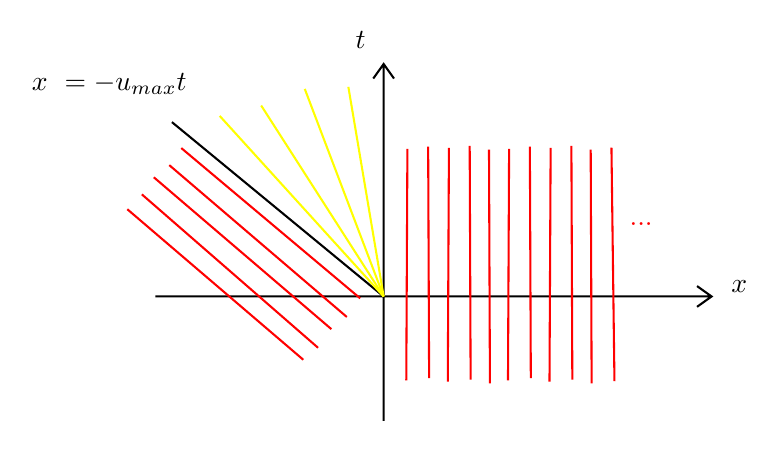
\begin{tikzpicture}[x=0.75pt,y=0.75pt,yscale=-1,xscale=1]
                    %uncomment if require: \path (0,300); %set diagram left start at 0, and has height of 300

                    %Shape: Axis 2D [id:dp3242275334401292] 
                    \draw  (130,150) -- (398,150)(240,38) -- (240,210) (391,145) -- (398,150) -- (391,155) (235,45) -- (240,38) -- (245,45)  ;
                    %Straight Lines [id:da02222492658014852] 
                    \draw [color={rgb, 255:red, 255; green, 0; blue, 0 }  ,draw opacity=1 ]   (319.91,191.02) -- (320.46,78.46) ;
                    %Straight Lines [id:da4338095240978027] 
                    \draw [color={rgb, 255:red, 255; green, 0; blue, 0 }  ,draw opacity=1 ]   (340.21,191.83) -- (339.76,79.27) ;
                    %Straight Lines [id:da7151116176791149] 
                    \draw [color={rgb, 255:red, 255; green, 0; blue, 0 }  ,draw opacity=1 ]   (299.91,190.39) -- (300.45,78.84) ;
                    %Straight Lines [id:da3794350886499228] 
                    \draw [color={rgb, 255:red, 255; green, 0; blue, 0 }  ,draw opacity=1 ]   (330.91,190.02) -- (330.46,77.46) ;
                    %Straight Lines [id:da6561401855095113] 
                    \draw [color={rgb, 255:red, 255; green, 0; blue, 0 }  ,draw opacity=1 ]   (351.21,190.83) -- (349.76,78.27) ;
                    %Straight Lines [id:da27040052523613545] 
                    \draw [color={rgb, 255:red, 255; green, 0; blue, 0 }  ,draw opacity=1 ]   (310.91,189.39) -- (310.45,77.84) ;
                    %Straight Lines [id:da43272068532874564] 
                    \draw [color={rgb, 255:red, 255; green, 0; blue, 0 }  ,draw opacity=1 ]   (270.91,191.02) -- (271.46,78.46) ;
                    %Straight Lines [id:da3447299153844853] 
                    \draw [color={rgb, 255:red, 255; green, 0; blue, 0 }  ,draw opacity=1 ]   (291.21,191.83) -- (290.76,79.27) ;
                    %Straight Lines [id:da09487745849680329] 
                    \draw [color={rgb, 255:red, 255; green, 0; blue, 0 }  ,draw opacity=1 ]   (250.91,190.39) -- (251.45,78.84) ;
                    %Straight Lines [id:da6111461950814078] 
                    \draw [color={rgb, 255:red, 255; green, 0; blue, 0 }  ,draw opacity=1 ]   (281.91,190.02) -- (281.46,77.46) ;
                    %Straight Lines [id:da9155729958220498] 
                    \draw [color={rgb, 255:red, 255; green, 0; blue, 0 }  ,draw opacity=1 ]   (261.91,189.39) -- (261.45,77.84) ;
                    %Straight Lines [id:da10353936092794236] 
                    \draw    (138,66) -- (240,150) ;
                    %Straight Lines [id:da8684112446016625] 
                    \draw [color={rgb, 255:red, 255; green, 0; blue, 0 }  ,draw opacity=1 ]   (208.4,174.72) -- (123.51,100.81) ;
                    %Straight Lines [id:da5352469293291663] 
                    \draw [color={rgb, 255:red, 255; green, 0; blue, 0 }  ,draw opacity=1 ]   (222.26,159.88) -- (136.73,86.73) ;
                    %Straight Lines [id:da5211199646319873] 
                    \draw [color={rgb, 255:red, 255; green, 0; blue, 0 }  ,draw opacity=1 ]   (214.82,165.74) -- (129.28,92.59) ;
                    %Straight Lines [id:da9407595491423938] 
                    \draw [color={rgb, 255:red, 255; green, 0; blue, 0 }  ,draw opacity=1 ]   (228.69,150.9) -- (142.5,78.5) ;
                    %Straight Lines [id:da12980266937388085] 
                    \draw [color={rgb, 255:red, 255; green, 0; blue, 0 }  ,draw opacity=1 ]   (201.29,180.49) -- (116.51,107.98) ;
                    %Straight Lines [id:da08886092608553076] 
                    \draw [color={rgb, 255:red, 255; green, 255; blue, 0 }  ,draw opacity=1 ]   (161,63) -- (240,150) ;
                    %Straight Lines [id:da1604666647621502] 
                    \draw [color={rgb, 255:red, 255; green, 255; blue, 0 }  ,draw opacity=1 ]   (181,58) -- (240,150) ;
                    %Straight Lines [id:da9931053519803237] 
                    \draw [color={rgb, 255:red, 255; green, 255; blue, 0 }  ,draw opacity=1 ]   (202,50) -- (240,150) ;
                    %Straight Lines [id:da02051653712381518] 
                    \draw [color={rgb, 255:red, 255; green, 255; blue, 0 }  ,draw opacity=1 ]   (223,49) -- (240,150) ;

                    % Text Node
                    \draw (406,141) node [anchor=north west][inner sep=0.75pt]   [align=left] {$\displaystyle x$};
                    % Text Node
                    \draw (225,21) node [anchor=north west][inner sep=0.75pt]   [align=left] {$\displaystyle t$};
                    % Text Node
                    \draw (357,113) node [anchor=north west][inner sep=0.75pt]   [align=left] {\textcolor[rgb]{1,0,0}{...}};
                    % Text Node
                    \draw (69,41) node [anchor=north west][inner sep=0.75pt]   [align=left] {$\displaystyle x\ =-u_{max} t$};


                    \end{tikzpicture}
                \end{center}
            \end{figure}
            Las líneas amarillas muestran dónde se pueden meter las ondas de rarefacción. La frontera está delimitada por 
            $x = 0$ y por $x = - u_{max} t$. De esta manera, los tramos son $x<-u_{max}t$, $-u_{max} t < x < 0$ y $x > 0$.
            De esta manera, las ondas de rarefacción son:
            $$\rho(t,x) = \begin{cases}
                \frac{1}{2} \rho_{max} \quad& x < -u_{max} t \\
                \frac{x}{t} \quad & -u_{max} t \leq x < 0 \\
                \rho_{max} \quad& x > 0
            \end{cases}$$
            \item $\rho_0(x) = \begin{cases}
                \rho_{max} \quad& x < 0 \\
                \frac{1}{2} \rho_{max} \quad& x > 0
            \end{cases}$
            El dato inicial es en este caso decreciente. Este dato inicial 
            se corresponde con una situación que se suele denominar como de luz verde (el semáforo pasa de rojo a verde). \\

            Es completamente análogo al anterior pero cambiando los sentidos de las desigualdades. En este caso no hay ondas de rarefacción:
            Utilizando el cambio anterior, tenemos 
            $$R_0(x) = \begin{cases}
                0 \quad& x > 0 \\
                -u_{max} \quad& x < 0
            \end{cases}$$
            y aplicando el Teorema \ref{teo:t2}, nos queda 
            $$R(t,x) = \begin{cases}
                0 \quad& x > - \frac{u_{max}}{2} t \\
                -u_{max} \quad& x < - \frac{u_{max}}{2} t
            \end{cases}$$
            Deshaciendo el cambio, en función de $\rho$ nos queda:
            $$\rho(t,x) = \begin{cases}
                \dfrac{\rho_{max}}{2} \quad& x > - \frac{u_{max}}{2} t \\
                \rho_{max} \quad& x < - \frac{u_{max}}{2} t
            \end{cases}$$
            \item $\rho_0(x) = \begin{cases}
                \rho_{max} \quad& x > 0 \\
                \frac{1}{2} \rho_{max} \quad& x < 0
            \end{cases}$
        \end{itemize}
    \end{enumerate}
\end{ejercicio}

% El lunes resolveremos los dos ejercicios. El que es un poco más complicado es el c)




